\documentclass[11pt]{article}
% =======================================================================
%   Shared style for CS 300 notes.
%   Usage: place `% =======================================================================
%   Shared style for CS 300 notes.
%   Usage: place `% =======================================================================
%   Shared style for CS 300 notes.
%   Usage: place `\input{../../notes-style.tex}` right after \documentclass
%   in each chapter's lectures.tex and notes.tex.
% =======================================================================

% ---- Layout -----------------------------------------------------------
\usepackage[margin=1in]{geometry}
\usepackage{parskip}        % space between paragraphs, no indent
\usepackage{microtype}      % subtle kerning/spacing improvements

% ---- Colors (muted palette, easy on light-sensitive eyes) -------------
\usepackage{xcolor}
\definecolor{pagebg}       {HTML}{FAF6F0}  % warm cream background
\definecolor{bodyfg}       {HTML}{3D3A36}  % warm dark gray body text
\definecolor{heading}      {HTML}{3D6A6B}  % muted teal
\definecolor{subheading}   {HTML}{5B7A9C}  % dusty blue
\definecolor{accent}       {HTML}{8A6B4A}  % warm tan
\definecolor{linkcol}      {HTML}{5B7A9C}  % same as subheading
\definecolor{mutedtext}    {HTML}{6B6560}  % secondary / caption text
\definecolor{rulecol}      {HTML}{C8BFB0}  % separator / rule

% Callout box palette
\definecolor{defnFrame}    {HTML}{9DB89B}  \definecolor{defnBack}    {HTML}{EEF2E8}
\definecolor{ideaFrame}    {HTML}{9FB4CD}  \definecolor{ideaBack}    {HTML}{E8EEF5}
\definecolor{warnFrame}    {HTML}{CFAE87}  \definecolor{warnBack}    {HTML}{F5EDDF}
\definecolor{noteFrame}    {HTML}{BFA6AE}  \definecolor{noteBack}    {HTML}{F2E8EE}
\definecolor{exFrame}      {HTML}{9FBDBD}  \definecolor{exBack}      {HTML}{E8F0F0}
\definecolor{codeBack}     {HTML}{F3EDE2}
\definecolor{codeBorder}   {HTML}{D4CBBA}
\definecolor{codeKeyword}  {HTML}{6B4F7A}
\definecolor{codeString}   {HTML}{8A6B4A}
\definecolor{codeComment}  {HTML}{8A857F}

% ---- Page background + base text color --------------------------------
\usepackage{pagecolor}
\pagecolor{pagebg}
\color{bodyfg}

% ---- Fonts ------------------------------------------------------------
\usepackage[T1]{fontenc}
\IfFileExists{libertine.sty}{%
    \usepackage{libertine}      % warm, readable serif
    \usepackage[scaled=0.95]{inconsolata}  % softer monospace
}{}

% ---- Hyperref ---------------------------------------------------------
\usepackage{hyperref}
\hypersetup{
    colorlinks=true,
    linkcolor=linkcol,
    urlcolor=linkcol,
    citecolor=linkcol,
    pdfborder={0 0 0},
}

% ---- Section styling --------------------------------------------------
\usepackage[explicit]{titlesec}
\titleformat{\section}
    {\color{heading}\Large\bfseries}
    {\color{heading}\thesection\hspace{0.6em}}{0pt}{#1}
\titleformat{\subsection}
    {\color{subheading}\large\bfseries}
    {\color{subheading}\thesubsection\hspace{0.5em}}{0pt}{#1}
\titleformat{\subsubsection}
    {\color{accent}\normalsize\bfseries}
    {\color{accent}\thesubsubsection\hspace{0.5em}}{0pt}{#1}
\titleformat{\paragraph}[runin]
    {\color{accent}\bfseries}{}{0pt}{#1.}

\titlespacing*{\section}{0pt}{1.6em}{0.6em}
\titlespacing*{\subsection}{0pt}{1.2em}{0.4em}

% ---- Enumerate / itemize spacing --------------------------------------
\usepackage{enumitem}
\setlist[itemize]{leftmargin=1.4em, itemsep=2pt, topsep=4pt}
\setlist[enumerate]{leftmargin=1.6em, itemsep=2pt, topsep=4pt}

% ---- Code listings ----------------------------------------------------
\usepackage{listings}
\lstdefinestyle{notescode}{
    backgroundcolor=\color{codeBack},
    basicstyle=\ttfamily\small\color{bodyfg},
    keywordstyle=\color{codeKeyword}\bfseries,
    stringstyle=\color{codeString},
    commentstyle=\color{codeComment}\itshape,
    frame=single,
    framesep=6pt,
    rulecolor=\color{codeBorder},
    showstringspaces=false,
    breaklines=true,
    xleftmargin=10pt,
    xrightmargin=10pt,
    aboveskip=8pt,
    belowskip=8pt,
}
\lstset{style=notescode}

% ---- Callout boxes (tcolorbox) ----------------------------------------
\usepackage[most]{tcolorbox}

\newtcolorbox{defnbox}[1][]{
    enhanced, breakable,
    colback=defnBack, colframe=defnFrame, coltitle=bodyfg,
    title={\bfseries Definition \textemdash\ #1},
    fonttitle=\bfseries,
    boxrule=0.5pt, arc=2pt, left=8pt, right=8pt, top=6pt, bottom=6pt,
    attach boxed title to top left={xshift=10pt, yshift=-6pt},
    boxed title style={colback=defnFrame, colframe=defnFrame, arc=2pt},
    before skip=8pt, after skip=8pt,
}
\newtcolorbox{ideabox}[1][]{
    enhanced, breakable,
    colback=ideaBack, colframe=ideaFrame, coltitle=bodyfg,
    title={\bfseries Key idea #1},
    boxrule=0.5pt, arc=2pt, left=8pt, right=8pt, top=6pt, bottom=6pt,
    attach boxed title to top left={xshift=10pt, yshift=-6pt},
    boxed title style={colback=ideaFrame, colframe=ideaFrame, arc=2pt},
    before skip=8pt, after skip=8pt,
}
\newtcolorbox{warnbox}[1][]{
    enhanced, breakable,
    colback=warnBack, colframe=warnFrame, coltitle=bodyfg,
    title={\bfseries Gotcha #1},
    boxrule=0.5pt, arc=2pt, left=8pt, right=8pt, top=6pt, bottom=6pt,
    attach boxed title to top left={xshift=10pt, yshift=-6pt},
    boxed title style={colback=warnFrame, colframe=warnFrame, arc=2pt},
    before skip=8pt, after skip=8pt,
}
\newtcolorbox{notebox}[1][]{
    enhanced, breakable,
    colback=noteBack, colframe=noteFrame, coltitle=bodyfg,
    title={\bfseries Aside #1},
    boxrule=0.5pt, arc=2pt, left=8pt, right=8pt, top=6pt, bottom=6pt,
    attach boxed title to top left={xshift=10pt, yshift=-6pt},
    boxed title style={colback=noteFrame, colframe=noteFrame, arc=2pt},
    before skip=8pt, after skip=8pt,
}
\newtcolorbox{examplebox}[1][]{
    enhanced, breakable,
    colback=exBack, colframe=exFrame, coltitle=bodyfg,
    title={\bfseries Example #1},
    boxrule=0.5pt, arc=2pt, left=8pt, right=8pt, top=6pt, bottom=6pt,
    attach boxed title to top left={xshift=10pt, yshift=-6pt},
    boxed title style={colback=exFrame, colframe=exFrame, arc=2pt},
    before skip=8pt, after skip=8pt,
}

% ---- TikZ graph styles (added 2026-04-25 for ch_10 augmentation) ------
% tcolorbox[most] already loads tikz; this block declares the libraries
% + shared `vertex` / `edge` styles used by ch_10's general directed-graph
% diagrams. ch_9's tree-style TikZ uses inline overrides and is
% unaffected. Simple circle nodes + arrow edges only -- no production
% styling.
\usetikzlibrary{arrows.meta, positioning, calc}
\tikzset{
    vertex/.style={circle, draw, minimum size=7mm, inner sep=0pt,
                   font=\small, thick},
    vsource/.style={vertex, fill=ideaBack},
    vdone/.style={vertex, fill=defnBack},
    edge/.style={->, >=Stealth, thick},
    uedge/.style={-, thick},
    treeedge/.style={->, >=Stealth, thick},
    backedge/.style={->, >=Stealth, thick, dashed, red!70!black},
    fwdedge/.style={->, >=Stealth, thick, blue!60!black},
    crossedge/.style={->, >=Stealth, thick, green!50!black, dotted},
    mstedge/.style={-, very thick, accent},
}

% ---- Title block ------------------------------------------------------
\usepackage{titling}
\pretitle{\begin{center}\color{heading}\LARGE\bfseries}
\posttitle{\end{center}\vskip -0.4em}
\preauthor{\begin{center}\color{mutedtext}\normalsize}
\postauthor{\end{center}}
\predate{\begin{center}\color{mutedtext}\small}
\postdate{\end{center}\vspace{0.4em}{\color{rulecol}\hrule height 0.4pt}\vspace{1.2em}}
` right after \documentclass
%   in each chapter's lectures.tex and notes.tex.
% =======================================================================

% ---- Layout -----------------------------------------------------------
\usepackage[margin=1in]{geometry}
\usepackage{parskip}        % space between paragraphs, no indent
\usepackage{microtype}      % subtle kerning/spacing improvements

% ---- Colors (muted palette, easy on light-sensitive eyes) -------------
\usepackage{xcolor}
\definecolor{pagebg}       {HTML}{FAF6F0}  % warm cream background
\definecolor{bodyfg}       {HTML}{3D3A36}  % warm dark gray body text
\definecolor{heading}      {HTML}{3D6A6B}  % muted teal
\definecolor{subheading}   {HTML}{5B7A9C}  % dusty blue
\definecolor{accent}       {HTML}{8A6B4A}  % warm tan
\definecolor{linkcol}      {HTML}{5B7A9C}  % same as subheading
\definecolor{mutedtext}    {HTML}{6B6560}  % secondary / caption text
\definecolor{rulecol}      {HTML}{C8BFB0}  % separator / rule

% Callout box palette
\definecolor{defnFrame}    {HTML}{9DB89B}  \definecolor{defnBack}    {HTML}{EEF2E8}
\definecolor{ideaFrame}    {HTML}{9FB4CD}  \definecolor{ideaBack}    {HTML}{E8EEF5}
\definecolor{warnFrame}    {HTML}{CFAE87}  \definecolor{warnBack}    {HTML}{F5EDDF}
\definecolor{noteFrame}    {HTML}{BFA6AE}  \definecolor{noteBack}    {HTML}{F2E8EE}
\definecolor{exFrame}      {HTML}{9FBDBD}  \definecolor{exBack}      {HTML}{E8F0F0}
\definecolor{codeBack}     {HTML}{F3EDE2}
\definecolor{codeBorder}   {HTML}{D4CBBA}
\definecolor{codeKeyword}  {HTML}{6B4F7A}
\definecolor{codeString}   {HTML}{8A6B4A}
\definecolor{codeComment}  {HTML}{8A857F}

% ---- Page background + base text color --------------------------------
\usepackage{pagecolor}
\pagecolor{pagebg}
\color{bodyfg}

% ---- Fonts ------------------------------------------------------------
\usepackage[T1]{fontenc}
\IfFileExists{libertine.sty}{%
    \usepackage{libertine}      % warm, readable serif
    \usepackage[scaled=0.95]{inconsolata}  % softer monospace
}{}

% ---- Hyperref ---------------------------------------------------------
\usepackage{hyperref}
\hypersetup{
    colorlinks=true,
    linkcolor=linkcol,
    urlcolor=linkcol,
    citecolor=linkcol,
    pdfborder={0 0 0},
}

% ---- Section styling --------------------------------------------------
\usepackage[explicit]{titlesec}
\titleformat{\section}
    {\color{heading}\Large\bfseries}
    {\color{heading}\thesection\hspace{0.6em}}{0pt}{#1}
\titleformat{\subsection}
    {\color{subheading}\large\bfseries}
    {\color{subheading}\thesubsection\hspace{0.5em}}{0pt}{#1}
\titleformat{\subsubsection}
    {\color{accent}\normalsize\bfseries}
    {\color{accent}\thesubsubsection\hspace{0.5em}}{0pt}{#1}
\titleformat{\paragraph}[runin]
    {\color{accent}\bfseries}{}{0pt}{#1.}

\titlespacing*{\section}{0pt}{1.6em}{0.6em}
\titlespacing*{\subsection}{0pt}{1.2em}{0.4em}

% ---- Enumerate / itemize spacing --------------------------------------
\usepackage{enumitem}
\setlist[itemize]{leftmargin=1.4em, itemsep=2pt, topsep=4pt}
\setlist[enumerate]{leftmargin=1.6em, itemsep=2pt, topsep=4pt}

% ---- Code listings ----------------------------------------------------
\usepackage{listings}
\lstdefinestyle{notescode}{
    backgroundcolor=\color{codeBack},
    basicstyle=\ttfamily\small\color{bodyfg},
    keywordstyle=\color{codeKeyword}\bfseries,
    stringstyle=\color{codeString},
    commentstyle=\color{codeComment}\itshape,
    frame=single,
    framesep=6pt,
    rulecolor=\color{codeBorder},
    showstringspaces=false,
    breaklines=true,
    xleftmargin=10pt,
    xrightmargin=10pt,
    aboveskip=8pt,
    belowskip=8pt,
}
\lstset{style=notescode}

% ---- Callout boxes (tcolorbox) ----------------------------------------
\usepackage[most]{tcolorbox}

\newtcolorbox{defnbox}[1][]{
    enhanced, breakable,
    colback=defnBack, colframe=defnFrame, coltitle=bodyfg,
    title={\bfseries Definition \textemdash\ #1},
    fonttitle=\bfseries,
    boxrule=0.5pt, arc=2pt, left=8pt, right=8pt, top=6pt, bottom=6pt,
    attach boxed title to top left={xshift=10pt, yshift=-6pt},
    boxed title style={colback=defnFrame, colframe=defnFrame, arc=2pt},
    before skip=8pt, after skip=8pt,
}
\newtcolorbox{ideabox}[1][]{
    enhanced, breakable,
    colback=ideaBack, colframe=ideaFrame, coltitle=bodyfg,
    title={\bfseries Key idea #1},
    boxrule=0.5pt, arc=2pt, left=8pt, right=8pt, top=6pt, bottom=6pt,
    attach boxed title to top left={xshift=10pt, yshift=-6pt},
    boxed title style={colback=ideaFrame, colframe=ideaFrame, arc=2pt},
    before skip=8pt, after skip=8pt,
}
\newtcolorbox{warnbox}[1][]{
    enhanced, breakable,
    colback=warnBack, colframe=warnFrame, coltitle=bodyfg,
    title={\bfseries Gotcha #1},
    boxrule=0.5pt, arc=2pt, left=8pt, right=8pt, top=6pt, bottom=6pt,
    attach boxed title to top left={xshift=10pt, yshift=-6pt},
    boxed title style={colback=warnFrame, colframe=warnFrame, arc=2pt},
    before skip=8pt, after skip=8pt,
}
\newtcolorbox{notebox}[1][]{
    enhanced, breakable,
    colback=noteBack, colframe=noteFrame, coltitle=bodyfg,
    title={\bfseries Aside #1},
    boxrule=0.5pt, arc=2pt, left=8pt, right=8pt, top=6pt, bottom=6pt,
    attach boxed title to top left={xshift=10pt, yshift=-6pt},
    boxed title style={colback=noteFrame, colframe=noteFrame, arc=2pt},
    before skip=8pt, after skip=8pt,
}
\newtcolorbox{examplebox}[1][]{
    enhanced, breakable,
    colback=exBack, colframe=exFrame, coltitle=bodyfg,
    title={\bfseries Example #1},
    boxrule=0.5pt, arc=2pt, left=8pt, right=8pt, top=6pt, bottom=6pt,
    attach boxed title to top left={xshift=10pt, yshift=-6pt},
    boxed title style={colback=exFrame, colframe=exFrame, arc=2pt},
    before skip=8pt, after skip=8pt,
}

% ---- TikZ graph styles (added 2026-04-25 for ch_10 augmentation) ------
% tcolorbox[most] already loads tikz; this block declares the libraries
% + shared `vertex` / `edge` styles used by ch_10's general directed-graph
% diagrams. ch_9's tree-style TikZ uses inline overrides and is
% unaffected. Simple circle nodes + arrow edges only -- no production
% styling.
\usetikzlibrary{arrows.meta, positioning, calc}
\tikzset{
    vertex/.style={circle, draw, minimum size=7mm, inner sep=0pt,
                   font=\small, thick},
    vsource/.style={vertex, fill=ideaBack},
    vdone/.style={vertex, fill=defnBack},
    edge/.style={->, >=Stealth, thick},
    uedge/.style={-, thick},
    treeedge/.style={->, >=Stealth, thick},
    backedge/.style={->, >=Stealth, thick, dashed, red!70!black},
    fwdedge/.style={->, >=Stealth, thick, blue!60!black},
    crossedge/.style={->, >=Stealth, thick, green!50!black, dotted},
    mstedge/.style={-, very thick, accent},
}

% ---- Title block ------------------------------------------------------
\usepackage{titling}
\pretitle{\begin{center}\color{heading}\LARGE\bfseries}
\posttitle{\end{center}\vskip -0.4em}
\preauthor{\begin{center}\color{mutedtext}\normalsize}
\postauthor{\end{center}}
\predate{\begin{center}\color{mutedtext}\small}
\postdate{\end{center}\vspace{0.4em}{\color{rulecol}\hrule height 0.4pt}\vspace{1.2em}}
` right after \documentclass
%   in each chapter's lectures.tex and notes.tex.
% =======================================================================

% ---- Layout -----------------------------------------------------------
\usepackage[margin=1in]{geometry}
\usepackage{parskip}        % space between paragraphs, no indent
\usepackage{microtype}      % subtle kerning/spacing improvements

% ---- Colors (muted palette, easy on light-sensitive eyes) -------------
\usepackage{xcolor}
\definecolor{pagebg}       {HTML}{FAF6F0}  % warm cream background
\definecolor{bodyfg}       {HTML}{3D3A36}  % warm dark gray body text
\definecolor{heading}      {HTML}{3D6A6B}  % muted teal
\definecolor{subheading}   {HTML}{5B7A9C}  % dusty blue
\definecolor{accent}       {HTML}{8A6B4A}  % warm tan
\definecolor{linkcol}      {HTML}{5B7A9C}  % same as subheading
\definecolor{mutedtext}    {HTML}{6B6560}  % secondary / caption text
\definecolor{rulecol}      {HTML}{C8BFB0}  % separator / rule

% Callout box palette
\definecolor{defnFrame}    {HTML}{9DB89B}  \definecolor{defnBack}    {HTML}{EEF2E8}
\definecolor{ideaFrame}    {HTML}{9FB4CD}  \definecolor{ideaBack}    {HTML}{E8EEF5}
\definecolor{warnFrame}    {HTML}{CFAE87}  \definecolor{warnBack}    {HTML}{F5EDDF}
\definecolor{noteFrame}    {HTML}{BFA6AE}  \definecolor{noteBack}    {HTML}{F2E8EE}
\definecolor{exFrame}      {HTML}{9FBDBD}  \definecolor{exBack}      {HTML}{E8F0F0}
\definecolor{codeBack}     {HTML}{F3EDE2}
\definecolor{codeBorder}   {HTML}{D4CBBA}
\definecolor{codeKeyword}  {HTML}{6B4F7A}
\definecolor{codeString}   {HTML}{8A6B4A}
\definecolor{codeComment}  {HTML}{8A857F}

% ---- Page background + base text color --------------------------------
\usepackage{pagecolor}
\pagecolor{pagebg}
\color{bodyfg}

% ---- Fonts ------------------------------------------------------------
\usepackage[T1]{fontenc}
\IfFileExists{libertine.sty}{%
    \usepackage{libertine}      % warm, readable serif
    \usepackage[scaled=0.95]{inconsolata}  % softer monospace
}{}

% ---- Hyperref ---------------------------------------------------------
\usepackage{hyperref}
\hypersetup{
    colorlinks=true,
    linkcolor=linkcol,
    urlcolor=linkcol,
    citecolor=linkcol,
    pdfborder={0 0 0},
}

% ---- Section styling --------------------------------------------------
\usepackage[explicit]{titlesec}
\titleformat{\section}
    {\color{heading}\Large\bfseries}
    {\color{heading}\thesection\hspace{0.6em}}{0pt}{#1}
\titleformat{\subsection}
    {\color{subheading}\large\bfseries}
    {\color{subheading}\thesubsection\hspace{0.5em}}{0pt}{#1}
\titleformat{\subsubsection}
    {\color{accent}\normalsize\bfseries}
    {\color{accent}\thesubsubsection\hspace{0.5em}}{0pt}{#1}
\titleformat{\paragraph}[runin]
    {\color{accent}\bfseries}{}{0pt}{#1.}

\titlespacing*{\section}{0pt}{1.6em}{0.6em}
\titlespacing*{\subsection}{0pt}{1.2em}{0.4em}

% ---- Enumerate / itemize spacing --------------------------------------
\usepackage{enumitem}
\setlist[itemize]{leftmargin=1.4em, itemsep=2pt, topsep=4pt}
\setlist[enumerate]{leftmargin=1.6em, itemsep=2pt, topsep=4pt}

% ---- Code listings ----------------------------------------------------
\usepackage{listings}
\lstdefinestyle{notescode}{
    backgroundcolor=\color{codeBack},
    basicstyle=\ttfamily\small\color{bodyfg},
    keywordstyle=\color{codeKeyword}\bfseries,
    stringstyle=\color{codeString},
    commentstyle=\color{codeComment}\itshape,
    frame=single,
    framesep=6pt,
    rulecolor=\color{codeBorder},
    showstringspaces=false,
    breaklines=true,
    xleftmargin=10pt,
    xrightmargin=10pt,
    aboveskip=8pt,
    belowskip=8pt,
}
\lstset{style=notescode}

% ---- Callout boxes (tcolorbox) ----------------------------------------
\usepackage[most]{tcolorbox}

\newtcolorbox{defnbox}[1][]{
    enhanced, breakable,
    colback=defnBack, colframe=defnFrame, coltitle=bodyfg,
    title={\bfseries Definition \textemdash\ #1},
    fonttitle=\bfseries,
    boxrule=0.5pt, arc=2pt, left=8pt, right=8pt, top=6pt, bottom=6pt,
    attach boxed title to top left={xshift=10pt, yshift=-6pt},
    boxed title style={colback=defnFrame, colframe=defnFrame, arc=2pt},
    before skip=8pt, after skip=8pt,
}
\newtcolorbox{ideabox}[1][]{
    enhanced, breakable,
    colback=ideaBack, colframe=ideaFrame, coltitle=bodyfg,
    title={\bfseries Key idea #1},
    boxrule=0.5pt, arc=2pt, left=8pt, right=8pt, top=6pt, bottom=6pt,
    attach boxed title to top left={xshift=10pt, yshift=-6pt},
    boxed title style={colback=ideaFrame, colframe=ideaFrame, arc=2pt},
    before skip=8pt, after skip=8pt,
}
\newtcolorbox{warnbox}[1][]{
    enhanced, breakable,
    colback=warnBack, colframe=warnFrame, coltitle=bodyfg,
    title={\bfseries Gotcha #1},
    boxrule=0.5pt, arc=2pt, left=8pt, right=8pt, top=6pt, bottom=6pt,
    attach boxed title to top left={xshift=10pt, yshift=-6pt},
    boxed title style={colback=warnFrame, colframe=warnFrame, arc=2pt},
    before skip=8pt, after skip=8pt,
}
\newtcolorbox{notebox}[1][]{
    enhanced, breakable,
    colback=noteBack, colframe=noteFrame, coltitle=bodyfg,
    title={\bfseries Aside #1},
    boxrule=0.5pt, arc=2pt, left=8pt, right=8pt, top=6pt, bottom=6pt,
    attach boxed title to top left={xshift=10pt, yshift=-6pt},
    boxed title style={colback=noteFrame, colframe=noteFrame, arc=2pt},
    before skip=8pt, after skip=8pt,
}
\newtcolorbox{examplebox}[1][]{
    enhanced, breakable,
    colback=exBack, colframe=exFrame, coltitle=bodyfg,
    title={\bfseries Example #1},
    boxrule=0.5pt, arc=2pt, left=8pt, right=8pt, top=6pt, bottom=6pt,
    attach boxed title to top left={xshift=10pt, yshift=-6pt},
    boxed title style={colback=exFrame, colframe=exFrame, arc=2pt},
    before skip=8pt, after skip=8pt,
}

% ---- TikZ graph styles (added 2026-04-25 for ch_10 augmentation) ------
% tcolorbox[most] already loads tikz; this block declares the libraries
% + shared `vertex` / `edge` styles used by ch_10's general directed-graph
% diagrams. ch_9's tree-style TikZ uses inline overrides and is
% unaffected. Simple circle nodes + arrow edges only -- no production
% styling.
\usetikzlibrary{arrows.meta, positioning, calc}
\tikzset{
    vertex/.style={circle, draw, minimum size=7mm, inner sep=0pt,
                   font=\small, thick},
    vsource/.style={vertex, fill=ideaBack},
    vdone/.style={vertex, fill=defnBack},
    edge/.style={->, >=Stealth, thick},
    uedge/.style={-, thick},
    treeedge/.style={->, >=Stealth, thick},
    backedge/.style={->, >=Stealth, thick, dashed, red!70!black},
    fwdedge/.style={->, >=Stealth, thick, blue!60!black},
    crossedge/.style={->, >=Stealth, thick, green!50!black, dotted},
    mstedge/.style={-, very thick, accent},
}

% ---- Title block ------------------------------------------------------
\usepackage{titling}
\pretitle{\begin{center}\color{heading}\LARGE\bfseries}
\posttitle{\end{center}\vskip -0.4em}
\preauthor{\begin{center}\color{mutedtext}\normalsize}
\postauthor{\end{center}}
\predate{\begin{center}\color{mutedtext}\small}
\postdate{\end{center}\vspace{0.4em}{\color{rulecol}\hrule height 0.4pt}\vspace{1.2em}}


\title{CS 300 -- Chapter 11 Lectures\\\large B-Trees}
\author{Jose de Lima}
\date{\today}

\begin{document}
\maketitle

\begin{ideabox}[Chapter map]
\textbf{Where this sits in CS 300.} Chapter 11 is the
\emph{shallow-and-wide tree chapter}. \textbf{ch.~9} covered AVL and
red-black trees as the canonical balanced \emph{binary} trees:
height $O(\log_2 n)$, every level branches by 2. Chapter 11
generalises to balanced \emph{$K$-ary} trees: height
$O(\log_K n)$, every level branches by $K$. The motivating shift
is the \textbf{memory hierarchy}. When each level of the tree is a
disk seek (10\,ms), DRAM cache miss (100\,ns), or NVMe read
(50\,$\mu$s), reducing height by a factor of $\log_2 K$ is enormous.
B-trees are why every modern database, filesystem, and key-value
store uses them; the production references at the end of this
chapter (\S11.7) are dense.

\textbf{What you add to your toolkit:}
\begin{itemize}
    \item \textbf{The minimum-degree parameter.} CLRS calls it $t$;
          these notes use \emph{order $K$} ($K = 2t$ in CLRS terms).
          The resulting \textbf{node-occupancy bounds}
          ($\lceil K/2 \rceil - 1$ to $K-1$ keys per non-root node;
          root exception) are the workhorse invariant the algorithms
          rely on.
    \item \textbf{Height bound} $h \le \log_t \frac{n+1}{2}$ ---
          derived from worst-case occupancy. This is why a B-tree of
          order 100 is only $\sim 5$ levels deep at $n = 10^9$.
    \item \textbf{Preemptive top-down split.} The single-pass
          insertion strategy that avoids the upward recursion a
          naive bottom-up split would force.
    \item \textbf{Preemptive merge.} The mirror: rotate-or-fuse on
          the way down so the leaf is always safe to delete from.
    \item \textbf{B+ trees.} The production refinement where data
          lives only at leaves and the leaves form a linked list ---
          this is what your database actually uses, and it's why
          range queries are cheap.
    \item \textbf{Where B-trees show up in production:} SQLite
          indexes, PostgreSQL (\texttt{btree} access method), MySQL
          InnoDB (clustered B+ tree on the primary key), Linux ext4
          (htree directory entries), Btrfs (copy-on-write B+ trees
          throughout), git packfile \texttt{.idx} (sorted-array, not
          B-tree --- a useful contrast), LSM-trees on top of B-trees
          (LevelDB, RocksDB, Cassandra).
\end{itemize}

\textbf{Mastery checklist} --- you should be able to, without
references:
\begin{enumerate}
    \item State the B-tree node-occupancy invariant
          ($\lceil K/2 \rceil - 1 \le \text{keys} \le K-1$, root
          excepted) and sketch why this gives $h = O(\log_K n)$.
    \item Run a B-tree search by hand on a 3-level tree of order
          $K=4$: identify the in-node scan + descent at each level
          (\S11.2).
    \item Walk through a preemptive top-down split insertion: insert
          into a tree where the descent path contains a full node,
          and identify how the split propagates the median key to
          the parent (\S11.3).
    \item Identify the four CLRS B-TREE-DELETE cases on a worked
          example: (1) key in leaf, (2) key in internal node with
          three subcases 2a/2b/2c, (3) key not in current node with
          subcases 3a/3b (\S11.4--\S11.5).
    \item Distinguish B-tree from B+ tree: data-at-internal-nodes
          vs data-at-leaves-only with a linked list of leaves;
          argue when the B+ form is preferable (range queries,
          sequential scans, \S11.5).
    \item Pick the right B-tree order $K$ for a given memory
          hierarchy. Page size + key+pointer size determine the
          target fanout (a 4\,KB page with 16-byte (key, pointer)
          slots gives $K \approx 256$; a 1\,KB page with 16-byte
          slots gives $K \approx 64$; \S11.1).
    \item State why B-trees beat hash tables for filesystem and
          database indexes (range queries, sequential scans,
          ordered iteration are all cheap on B-trees and impossible
          on hash tables; \S11.7).
\end{enumerate}

\textbf{Looking ahead.} \textbf{Chapter 12} covers the \emph{set ADT}
in full; B-trees and B+ trees are the disk-side implementation
choice when persistence + ordered iteration matter (Java
\texttt{TreeMap} / C++ \texttt{std::set} use red-black; SQLite /
PostgreSQL / InnoDB use B+ trees for the same operations). The
production-database / systems-programming follow-on direction
beyond cs-300 lives in \S11.6 (cache-oblivious B-trees, LSM-trees,
fractal trees) and \S11.7 (the canonical references).
\end{ideabox}

\begin{ideabox}
\textbf{Why B-trees exist.} AVL and red-black trees (ch.\ 9) optimize for in-memory comparisons: each node holds one key and two children. But when your tree doesn't fit in RAM -- when it lives on disk or across a network -- a binary tree is a disaster. Each node traversal is a separate I/O operation. A tree of a billion keys is $\log_2 10^9 \approx 30$ levels deep; that's 30 disk seeks per lookup at roughly 10ms each = 300ms per query. A B-tree of the same size is $\log_{100} 10^9 \approx 4.5$ levels deep. Fatter nodes, fewer levels, fewer I/Os. \emph{B-trees are what happens when you let cache lines or disk blocks dictate your node size.}
\end{ideabox}

\section{11.1 B-tree Structure}

\subsection*{The definition}

\begin{defnbox}
\textbf{B-tree of order $K$.} A search tree where every node holds at most $K-1$ keys and at most $K$ children. Subject to:
\begin{itemize}[leftmargin=*]
    \item All keys in a node are stored in sorted order.
    \item An internal node with $n$ keys has exactly $n+1$ children.
    \item Between two adjacent keys, the child subtree holds keys strictly between them; outside the first or last key, the outer subtrees hold keys strictly less / greater.
    \item All leaves sit at the same depth. (This is the balance condition.)
    \item \textbf{Minimum-occupancy floor.} Every internal node \emph{except the root} holds at least $\lceil K/2 \rceil - 1$ keys (equivalently, at least $\lceil K/2 \rceil$ children). The root is exempt: it may carry as few as $1$ key (or $0$ keys when the tree is empty) and as many as $K-1$.
    \item All keys are distinct.
\end{itemize}
\end{defnbox}

\begin{notebox}
Different textbooks use subtly different definitions of ``order'' -- some count maximum children ($K$), some count maximum keys ($K-1$), some use a \emph{minimum} degree $t$ with $t-1$ to $2t-1$ keys per node. These notes use ``order $K$ = max children.'' In the CLRS convention, $K = 2t$, so the minimum-keys floor $\lceil K/2 \rceil - 1$ becomes $t - 1$ and the maximum is $2t - 1$. Translate carefully if you cross-reference CLRS or Knuth.
\end{notebox}

\begin{notebox}
\textbf{Root exception.} The minimum-keys floor is the workhorse invariant for most of the algorithms in this chapter --- preemptive split, preemptive merge, fusion, rotation all assume that any node we touch except the root has $\ge \lceil K/2 \rceil - 1$ keys. The root is special on both ends: when the tree is small the root may carry just one key (or be a leaf), and when the tree is empty the root pointer can be \texttt{nullptr}. \emph{Root-split} (\S11.3) and \emph{root-fusion} (\S11.4) are the two events that propagate height changes through this exception.
\end{notebox}

\subsection*{The 2-3-4 tree -- a B-tree of order 4}

Order-4 B-trees are the standard teaching example. A node holds:
\begin{itemize}[leftmargin=*]
    \item 1, 2, or 3 keys -- called \textbf{2-node}, \textbf{3-node}, or \textbf{4-node}.
    \item Correspondingly 2, 3, or 4 children (for internal nodes).
\end{itemize}

A common convention labels node keys as $A$, $B$, $C$ and children as \texttt{left}, \texttt{middle1}, \texttt{middle2}, \texttt{right}:

\begin{center}
\begin{tabular}{lll}
\hline
Node type & Keys used & Children used \\
\hline
2-node & $A$ & \texttt{left}, \texttt{middle1} \\
3-node & $A, B$ & \texttt{left}, \texttt{middle1}, \texttt{middle2} \\
4-node (full) & $A, B, C$ & \texttt{left}, \texttt{middle1}, \texttt{middle2}, \texttt{right} \\
\hline
\end{tabular}
\end{center}

\begin{ideabox}
2-3-4 trees are a finger exercise. Real B-trees in databases use orders in the hundreds or thousands -- typically whatever fits in one disk page (4KB--16KB) or one L2 cache line (a few hundred integers). The \emph{algorithms} are identical to the order-4 version; only the array sizes change.
\end{ideabox}

\subsection*{C++ node skeleton}

\begin{lstlisting}[basicstyle=\ttfamily\small,frame=single]
template<int Order>   // e.g. Order=4 for 2-3-4 trees
struct BTreeNode {
    int numKeys = 0;
    int keys[Order - 1];
    BTreeNode* children[Order] = {};     // null for leaves
    BTreeNode* parent = nullptr;

    bool isLeaf() const { return children[0] == nullptr; }
    bool isFull() const { return numKeys == Order - 1; }
};

template<int Order>
struct BTree {
    BTreeNode<Order>* root = nullptr;
};
\end{lstlisting}

\subsection*{Helper primitives}

The insert / remove / rotate / fuse listings later in this chapter
call into a small set of in-node primitives. We collect their
signatures + brief implementations here so the chapter listings are
runnable-shape rather than illustrative-only:

\begin{lstlisting}[basicstyle=\ttfamily\small,frame=single]
// Linear-scan key lookup inside one node. Returns -1 on miss.
template<int Order>
int indexOfKey(BTreeNode<Order>* n, int key) {
    for (int i = 0; i < n->numKeys; ++i)
        if (n->keys[i] == key) return i;
    return -1;
}
template<int Order>
bool containsKey(BTreeNode<Order>* n, int key) {
    return indexOfKey(n, key) != -1;
}

// Pick the child whose subtree must contain `key` (caller guarantees
// the key is not in `n` itself).
template<int Order>
BTreeNode<Order>* btreeChildForKey(BTreeNode<Order>* n, int key) {
    int i = 0;
    while (i < n->numKeys && key > n->keys[i]) ++i;
    return n->children[i];
}

// Insert `key` into a non-full leaf. Shifts existing keys right.
template<int Order>
void btreeInsertIntoLeaf(BTreeNode<Order>* n, int key) {
    int i = n->numKeys - 1;
    while (i >= 0 && n->keys[i] > key) {
        n->keys[i+1] = n->keys[i]; --i;
    }
    n->keys[i+1] = key; ++n->numKeys;
}

// Insert (key, leftChild, rightChild) into a non-full internal node,
// preserving sort order. Used by btreeSplit on the parent.
template<int Order>
void btreeInsertKeyWithChildren(BTreeNode<Order>* p, int key,
                                BTreeNode<Order>* L, BTreeNode<Order>* R) {
    int i = p->numKeys - 1;
    while (i >= 0 && p->keys[i] > key) {
        p->keys[i+1]      = p->keys[i];
        p->children[i+2]  = p->children[i+1];
        --i;
    }
    p->keys[i+1]     = key;
    p->children[i+1] = L;
    p->children[i+2] = R;
    ++p->numKeys;
    L->parent = R->parent = p;
}

// Drop key at index `idx`, shifting neighbours left.
template<int Order>
void removeKey(BTreeNode<Order>* n, int idx) {
    for (int i = idx; i < n->numKeys - 1; ++i)
        n->keys[i] = n->keys[i+1];
    --n->numKeys;
}

// Smallest key in the subtree rooted at `n` (leftmost descendant).
template<int Order>
int btreeGetMinKey(BTreeNode<Order>* n) {
    while (!n->isLeaf()) n = n->children[0];
    return n->keys[0];
}
\end{lstlisting}

\noindent The split / rotate / merge / fuse / remove listings later
treat the helpers above as black-box primitives. Production B-tree
code factors them similarly --- the algorithm-level listings stay
readable, the in-node bookkeeping lives in one place.

\subsection*{The CLRS minimum-degree convention --- $t$ vs $K$}

\begin{notebox}
\textbf{$t \leftrightarrow K$ bridge.} CLRS Ch.~18 parameterises
B-trees by a \emph{minimum degree} $t \ge 2$: every internal node
except the root has at least $t-1$ keys and at most $2t-1$ keys
(equivalently, between $t$ and $2t$ children). Order $K$ as defined
above relates by $K = 2t$, so:
\begin{itemize}[leftmargin=*]
    \item Min keys per non-root: $\lceil K/2 \rceil - 1 = t - 1$.
    \item Max keys per node: $K - 1 = 2t - 1$.
    \item Min children per non-root: $\lceil K/2 \rceil = t$.
    \item Max children per node: $K = 2t$.
\end{itemize}
The 2-3-4 tree has $t = 2$, $K = 4$: $1$ to $3$ keys, $2$ to $4$
children. Read \emph{order} as ``what's the maximum branching?''
and \emph{minimum degree} as ``what's the slack-to-merge
threshold?''; both encode the same bounds.
\end{notebox}

\subsection*{Height analysis}

A B-tree of order $K$ with $n$ keys has height $h = O(\log_K n)$. For $K = 100$ and $n = 10^9$, that's $\log_{100} 10^9 \approx 4.5$ -- roughly 5 node accesses per lookup. Contrast with a binary tree's $\log_2 10^9 \approx 30$.

That factor-of-six reduction is the whole point. On disk it translates directly to query latency.

\begin{defnbox}
\textbf{Height bound (CLRS Theorem 18.1).} If $n \ge 1$ keys live in
a B-tree $T$ of minimum degree $t \ge 2$, then
\[
    h \;\le\; \log_t \frac{n+1}{2}.
\]
\textbf{Sketch.} Worst case: every node hits the minimum-occupancy
floor (root has 1 key, every other node has $t-1$ keys). Counting
nodes per level:
\begin{itemize}[leftmargin=*]
    \item Level 0 (root): $1$ node.
    \item Level 1: $\ge 2$ nodes (root has 2 children minimum).
    \item Level 2: $\ge 2t$ nodes (each level-1 node has $\ge t$
          children).
    \item Level $i \ge 1$: $\ge 2t^{i-1}$ nodes.
\end{itemize}
Each node holds at least $t-1$ keys, plus the root contributes 1 key,
so
\[
    n \;\ge\; 1 + (t-1) \sum_{i=1}^{h} 2t^{i-1}
        \;=\; 1 + 2(t-1) \cdot \frac{t^h - 1}{t-1}
        \;=\; 2t^h - 1.
\]
Solving: $t^h \le (n+1)/2$, hence $h \le \log_t \frac{n+1}{2}$.\hfill\textbf{Q.E.D.}
\end{defnbox}

\subsection*{The disk-access cost model}

\begin{defnbox}
\textbf{Disk-access model (DAM).} The B-tree cost model of record.
Memory is partitioned into a small \emph{internal} buffer (DRAM,
$M$ words) and an unbounded \emph{external} store (disk, page size
$B$ words). Computation on internal data is free; the only cost
counted is \textbf{block transfers} between the two. A B-tree of
order $K$ tuned so one node = one disk page achieves
$\Theta(\log_K n) = \Theta(\log_B n)$ block transfers per
search / insert / delete --- and that's the whole point of the
data structure.
\end{defnbox}

\begin{notebox}
\textbf{Concrete sizing.} Pick $K$ so one node fills the underlying
block size. A few worked examples:
\begin{itemize}[leftmargin=*]
    \item \textbf{1\,KB page, 8-byte keys + 8-byte child pointers}
          $\Rightarrow$ each (key, pointer) slot is 16 bytes,
          $K \approx 1024 / 16 = 64$.
    \item \textbf{4\,KB page, same slot size} $\Rightarrow$
          $K \approx 256$. SQLite's default.
    \item \textbf{16\,KB page} (MySQL InnoDB default, PostgreSQL
          configurable) $\Rightarrow$ $K \approx 1024$, height
          $\le 4$ for $n = 10^{12}$.
    \item \textbf{64-byte cache line, 16-byte slots} $\Rightarrow$
          $K \approx 4$. The 2-3-4 register comes back when your
          ``page'' is a cache line --- relevant for in-memory
          $B$-trees in modern OLTP engines.
\end{itemize}
The take-away: $K$ is set by hardware geometry, not by any
algorithmic constraint. Pick the largest $K$ that keeps a node in
one block.
\end{notebox}

\subsection*{A 3-level B-tree of order 4 --- the running picture}

The structural invariants are easier to internalise on a worked
diagram. Below is a 3-level B-tree of order $K = 4$ (so 1--3 keys
per node, 2--4 children, leaves at the same depth):

\begin{center}
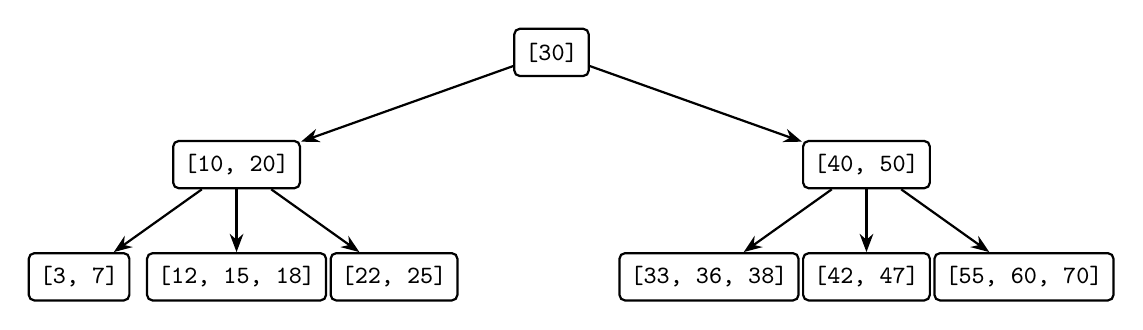
\begin{tikzpicture}[
    btnode/.style={draw, thick, rectangle, rounded corners=2pt,
                   inner sep=4pt, font=\small\ttfamily,
                   minimum height=6mm},
    btedge/.style={->, >=Stealth, thick},
    yscale=0.95,
]
% Root: a single 2-node holding 30 (1 key, 2 children).
\node[btnode] (root) at (0, 3) {[30]};
% Level 1: two internal 3-nodes.
\node[btnode] (n1) at (-4, 1.5) {[10, 20]};
\node[btnode] (n2) at ( 4, 1.5) {[40, 50]};
% Level 2: six leaves.
\node[btnode] (l1) at (-6,   0) {[3, 7]};
\node[btnode] (l2) at (-4,   0) {[12, 15, 18]};
\node[btnode] (l3) at (-2,   0) {[22, 25]};
\node[btnode] (l4) at ( 2,   0) {[33, 36, 38]};
\node[btnode] (l5) at ( 4,   0) {[42, 47]};
\node[btnode] (l6) at ( 6,   0) {[55, 60, 70]};
% Edges.
\draw[btedge] (root) -- (n1);
\draw[btedge] (root) -- (n2);
\draw[btedge] (n1) -- (l1);
\draw[btedge] (n1) -- (l2);
\draw[btedge] (n1) -- (l3);
\draw[btedge] (n2) -- (l4);
\draw[btedge] (n2) -- (l5);
\draw[btedge] (n2) -- (l6);
\end{tikzpicture}
\end{center}

Read off each invariant on the picture:
\begin{itemize}[leftmargin=*]
    \item \textbf{Sorted within node.} Every node's keys are
          left-to-right ascending: \texttt{[10, 20]},
          \texttt{[12, 15, 18]}, \texttt{[33, 36, 38]}.
    \item \textbf{$n+1$ children.} The root has 1 key, 2 children.
          \texttt{[10, 20]} has 2 keys, 3 children. The 4-node
          \texttt{[33, 36, 38]} would have 4 children if it were
          internal --- here it's a leaf.
    \item \textbf{Subtree key-ranges.} Under \texttt{[10, 20]}:
          left child is $< 10$ (\texttt{[3, 7]}), middle child is
          between 10 and 20 (\texttt{[12, 15, 18]}), right child is
          $> 20$ (\texttt{[22, 25]}).
    \item \textbf{All leaves at the same depth.} Every leaf sits at
          depth 2.
    \item \textbf{Min-occupancy floor.} Order $K = 4$
          $\Rightarrow$ $\lceil 4/2 \rceil - 1 = 1$ key minimum per
          non-root. Every non-root node holds $\ge 1$ key. Root
          exception: \texttt{[30]} has exactly 1 key (legal because
          it's the root).
\end{itemize}

This tree carries 16 keys at depth 3. With $K = 100$ on the same 3
levels, a B-tree carries up to $100^3 = 10^6$ keys --- the same
shape, vastly more capacity.

\begin{examplebox}
\textbf{Where B-trees actually live.}
\begin{itemize}[leftmargin=*]
    \item \textbf{Database indexes}: MySQL (InnoDB), PostgreSQL, SQL Server, Oracle all use B+ trees (a B-tree variant) for their default index structures.
    \item \textbf{Filesystems}: ext4, NTFS, HFS+, APFS, Btrfs (the ``B'' is for B-tree), XFS -- all B-tree-based for directory and extent management.
    \item \textbf{Key-value stores}: BoltDB, LMDB use B+ trees.
    \item \textbf{Version control}: Git's packfile index uses a B-tree-like structure for fast object lookup.
\end{itemize}
You won't ``implement a B-tree for production'' very often, but you'll read about them in every system's architecture doc.
\end{examplebox}

\section{11.2 Search}

\subsection*{The algorithm}

B-tree search is binary search \emph{within} a node combined with tree descent. At each node:
\begin{enumerate}[leftmargin=*]
    \item Linear-scan (or binary-search, for larger orders) the node's keys for the target.
    \item If found, return the node.
    \item Otherwise, find the child whose key range contains the target, and recurse.
\end{enumerate}

For the 2-3-4 case, the child selection reduces to a short comparison chain:

\begin{center}
\begin{tabular}{ll}
\hline
Condition & Descend to \\
\hline
key $<$ node.A & \texttt{left} \\
node has 1 key, or key $<$ node.B & \texttt{middle1} \\
node has 2 keys, or key $<$ node.C & \texttt{middle2} \\
otherwise & \texttt{right} \\
\hline
\end{tabular}
\end{center}

\begin{lstlisting}[basicstyle=\ttfamily\small,frame=single]
BTreeNode* btreeSearch(BTreeNode* node, int key) {
    if (!node) return nullptr;

    // Check keys in this node.
    if (node->numKeys >= 1 && node->keys[0] == key) return node;
    if (node->numKeys >= 2 && node->keys[1] == key) return node;
    if (node->numKeys >= 3 && node->keys[2] == key) return node;

    // Descend to the appropriate child.
    if (key < node->keys[0])
        return btreeSearch(node->children[0], key);     // left
    if (node->numKeys == 1 || key < node->keys[1])
        return btreeSearch(node->children[1], key);     // middle1
    if (node->numKeys == 2 || key < node->keys[2])
        return btreeSearch(node->children[2], key);     // middle2
    return btreeSearch(node->children[3], key);         // right
}
\end{lstlisting}

\subsection*{B-TREE-SEARCH --- the general form}

The 2-3-4-special listing above unrolls the in-node comparisons by
hand. CLRS Ch.~18.1 gives the general recursive form that works for
any order $K$: scan the keys for the smallest one $\ge$ the target,
either return on a hit or descend into the matching child.

\begin{lstlisting}[basicstyle=\ttfamily\small,frame=single]
template<int Order>
BTreeNode<Order>* btreeSearchGeneric(BTreeNode<Order>* node, int key) {
    if (!node) return nullptr;
    int i = 0;
    while (i < node->numKeys && key > node->keys[i]) ++i;
    if (i < node->numKeys && node->keys[i] == key) return node;
    if (node->isLeaf()) return nullptr;
    return btreeSearchGeneric(node->children[i], key);
}
\end{lstlisting}

\begin{notebox}
\textbf{Linear vs binary in-node scan.} The listing above uses a
linear scan (\texttt{while (key > keys[i])}). For small $K$ that's
optimal --- branch prediction and the linear-scan-fits-in-a-cache-line
property dominate the asymptotics. CLRS uses linear in pseudocode for
clarity. Production code with $K$ in the hundreds or thousands swaps
in a binary search inside the node:
\begin{lstlisting}[basicstyle=\ttfamily\small,frame=single]
int lo = 0, hi = node->numKeys;
while (lo < hi) {
    int mid = (lo + hi) / 2;
    if (node->keys[mid] < key) lo = mid + 1;
    else                       hi = mid;
}
\end{lstlisting}
giving $O(\log K)$ per-node CPU. The choice doesn't change the
disk-cost calculus --- both still touch one node per level.
\end{notebox}

\subsection*{Cost --- CPU vs disk decomposition}

\begin{center}
\begin{tabular}{lll}
\hline
Cost dimension & Linear in-node scan & Binary in-node scan \\
\hline
Disk reads (block transfers) & $O(\log_K n)$ & $O(\log_K n)$ \\
CPU comparisons / node       & $O(K)$        & $O(\log K)$    \\
Total CPU work               & $O(K \log_K n)$ & $O(\log K \cdot \log_K n) = O(\log n)$ \\
Memory accesses              & 1 per node-step & 1 per node-step \\
\hline
\end{tabular}
\end{center}

The two takeaways:
\begin{itemize}[leftmargin=*]
    \item \textbf{Disk cost is independent of in-node search style.}
          Both linear and binary read the same number of blocks ---
          one per level. That's what fanout buys you.
    \item \textbf{CPU cost equals balanced-binary-tree cost} once
          you switch to binary in-node search:
          $O(\log K \cdot \log_K n) = O(\log_2 n)$. So a B-tree is
          \emph{never} CPU-slower than a binary tree (on identical
          data) and is dramatically faster on disk-bound workloads.
\end{itemize}

\begin{ideabox}
Big-O hides the real win. A binary tree and a B-tree both do $O(\log n)$ comparisons, but the B-tree does them with one-tenth the \emph{pointer dereferences}. When each pointer dereference is a cache miss (or a disk seek), that's a 10$\times$ speedup, even though the asymptotic complexity is identical.
\end{ideabox}

\section{11.3 Insertion}

\subsection*{The big picture}

New keys always go into leaf nodes. The challenge: leaves might already be full. Strategy:

\begin{ideabox}
\textbf{Preemptive split.} As we descend from the root to the target leaf, \emph{split any full node we encounter along the way}. This guarantees the target leaf has room. Splits never cascade up, because every ancestor we visited is already non-full (we would have split it if not).
\end{ideabox}

\begin{notebox}
\textbf{Why preemptive top-down (and not retroactive bottom-up)?} The
``obvious'' algorithm is: descend to the leaf, insert, and if the
leaf overflows, split it and propagate the median key up to the
parent --- recursively splitting ancestors that overflow. That's
Knuth's classical algorithm. It works, but it requires either a
\textbf{second pass} from leaf back up to root or \textbf{parent
pointers} on every node so the recursion can return its way up.

CLRS Ch.~18.2 (and these notes) take the dual view: split any full
node \emph{before} descending into it. The invariant ``the current
node has room'' is preserved at every step of the recursion, so a
single downward pass suffices. The cost is splitting some nodes that
might not have actually needed it (you could've descended through a
full node without overflowing anything below) --- but the algorithmic
simplification is enormous: no upward recursion, no parent pointers
required, no second pass. The ``wasted work'' is bounded: at most
one split per level of the tree, so $O(\log_K n)$ extra work per
insert in the worst case.
\end{notebox}

\subsection*{The split operation}

A full node (with its maximum $K-1$ keys) is split into two nodes of $(K/2 - 1)$ keys each, and the middle key is promoted to the parent. For 2-3-4 trees:

\begin{center}
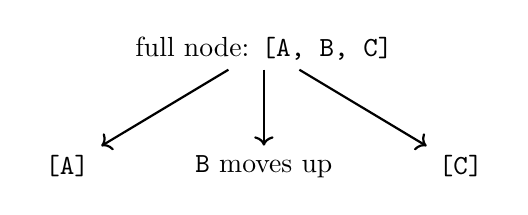
\begin{tikzpicture}[every node/.style={minimum width=1cm, minimum height=0.5cm}]
\node (src) at (0, 1.5) {full node: \texttt{[A, B, C]}};
\node (a) at (-2.5, 0) {\texttt{[A]}};
\node (parent) at (0, 0) {\texttt{B} moves up};
\node (c) at (2.5, 0) {\texttt{[C]}};
\draw[->, thick] (src) -- (a);
\draw[->, thick] (src) -- (parent);
\draw[->, thick] (src) -- (c);
\end{tikzpicture}
\end{center}

Keys $A$ and $C$ become two new sibling nodes; key $B$ moves into the parent, with pointers to the new siblings. The parent must have room (thanks to preemptive split).

\begin{lstlisting}[basicstyle=\ttfamily\small,frame=single]
BTreeNode* btreeSplit(BTree& t, BTreeNode* node) {
    if (!node->isFull()) return nullptr;
    BTreeNode* parent = node->parent;
    BTreeNode* left  = new BTreeNode{1, {node->keys[0]},
                                     {node->children[0], node->children[1]},
                                     parent};
    BTreeNode* right = new BTreeNode{1, {node->keys[2]},
                                     {node->children[2], node->children[3]},
                                     parent};

    if (parent) {
        btreeInsertKeyWithChildren(parent, node->keys[1], left, right);
    } else {
        parent = new BTreeNode{1, {node->keys[1]}, {left, right}, nullptr};
        t.root = parent;
        left->parent = right->parent = parent;
    }
    return parent;
}
\end{lstlisting}

\subsection*{B-TREE-SPLIT-CHILD --- the CLRS form}

The listing above is hard-coded to order 4. CLRS Ch.~18.2's
B-TREE-SPLIT-CHILD generalises to any order. The invariant: the
parent $p$ is non-full (so it has room for one more key + child
pointer), and the child to split is at index $i$. The child is full
($K-1$ keys); after the split, we get two siblings each with
$\lfloor (K-1)/2 \rfloor$ keys, and the median key moves up to $p$.

\begin{lstlisting}[basicstyle=\ttfamily\small,frame=single]
template<int Order>
void btreeSplitChild(BTreeNode<Order>* p, int i) {
    constexpr int t = Order / 2;          // CLRS minimum-degree t
    BTreeNode<Order>* y = p->children[i];  // the full child
    BTreeNode<Order>* z = new BTreeNode<Order>{};

    // z gets y's right half (keys [t .. 2t-2], children [t .. 2t-1]).
    z->numKeys = t - 1;
    for (int j = 0; j < t - 1; ++j)
        z->keys[j] = y->keys[j + t];
    if (!y->isLeaf()) {
        for (int j = 0; j < t; ++j) {
            z->children[j] = y->children[j + t];
            z->children[j]->parent = z;
            y->children[j + t] = nullptr;
        }
    }
    y->numKeys = t - 1;                   // y keeps left half

    // Make room in p for the new key + child pointer at slot i.
    for (int j = p->numKeys; j > i; --j)
        p->children[j + 1] = p->children[j];
    p->children[i + 1] = z;
    z->parent = p;
    for (int j = p->numKeys - 1; j >= i; --j)
        p->keys[j + 1] = p->keys[j];
    p->keys[i] = y->keys[t - 1];          // promote median
    ++p->numKeys;
}
\end{lstlisting}

\subsection*{B-TREE-INSERT-NONFULL --- the recursive descent}

CLRS Ch.~18.2 splits the insert API in two: \texttt{btreeInsert}
handles the root-split-as-only-height-growth event; everything else
goes through \texttt{btreeInsertNonFull}, which assumes the node it's
called on already has room. This is the cleanest expression of the
preemptive-split invariant.

\begin{lstlisting}[basicstyle=\ttfamily\small,frame=single]
template<int Order>
void btreeInsertNonFull(BTreeNode<Order>* node, int key) {
    int i = node->numKeys - 1;
    if (node->isLeaf()) {
        // Shift keys right, place new key in sorted slot.
        while (i >= 0 && node->keys[i] > key) {
            node->keys[i + 1] = node->keys[i]; --i;
        }
        node->keys[i + 1] = key;
        ++node->numKeys;
    } else {
        // Find child whose subtree contains key.
        while (i >= 0 && node->keys[i] > key) --i;
        ++i;
        // Preemptive split: if descent target is full, split first.
        if (node->children[i]->isFull()) {
            btreeSplitChild(node, i);
            // After split, decide which of the two halves to descend.
            if (key > node->keys[i]) ++i;
        }
        btreeInsertNonFull(node->children[i], key);
    }
}

template<int Order>
void btreeInsertCLRS(BTree<Order>& t, int key) {
    if (!t.root) { t.root = new BTreeNode<Order>{}; }
    if (t.root->isFull()) {
        // Root split: brand-new root, height grows by 1.
        BTreeNode<Order>* s = new BTreeNode<Order>{};
        s->children[0] = t.root;
        t.root->parent = s;
        t.root = s;
        btreeSplitChild(s, 0);
    }
    btreeInsertNonFull(t.root, key);
}
\end{lstlisting}

\noindent The split-and-shift bookkeeping is fiddly because the
arrays are fixed-size --- everything is in-place index arithmetic.
The algorithmic shape is identical to the order-4 \texttt{btreeSplit}
above; only the loop bounds change.

\subsection*{Special case: splitting the root}

When the root itself is full and we start inserting, the split creates a brand-new root with a single key. \textbf{This is the only way a B-tree grows in height.} Every other operation happens at the leaf level or via splits that push keys sideways to a non-full ancestor.

\begin{ideabox}
B-trees grow from the \emph{top} (via root splits), unlike binary search trees which grow from the bottom. That's why all leaves stay at the same depth -- depth increases uniformly when the root splits.
\end{ideabox}

\subsection*{Insert into a leaf}

Once we've descended (splitting along the way) to the target leaf, the leaf is guaranteed non-full. Insert the new key in sorted position:

\begin{center}
\begin{tabular}{ll}
\hline
Condition (non-full leaf) & Action \\
\hline
key equals existing key & no-op (duplicates forbidden) \\
key $<$ node.A & shift existing keys right, place new key at $A$ \\
key $<$ node.B (or no $B$) & shift $B \to C$ if needed, place new key at $B$ \\
otherwise & place new key at $C$ \\
\hline
\end{tabular}
\end{center}

\subsection*{The full insert}

\begin{lstlisting}[basicstyle=\ttfamily\small,frame=single]
BTreeNode* btreeInsert(BTreeNode* node, int key) {
    if (containsKey(node, key)) return nullptr;   // duplicates rejected

    if (node->isFull()) node = btreeSplit(node);  // preemptive split

    if (!node->isLeaf()) {
        BTreeNode* child = btreeChildForKey(node, key);
        return btreeInsert(child, key);
    }
    btreeInsertIntoLeaf(node, key);
    return node;
}
\end{lstlisting}

\subsection*{Cost}

\begin{itemize}[leftmargin=*]
    \item Descent: $O(\log_K n)$ levels.
    \item At each level: at most one split, $O(K)$ work.
    \item Total: $O(K \log_K n)$. For fixed $K$, that's $O(\log n)$.
\end{itemize}

\begin{warnbox}
\textbf{The ``lazy'' alternative.} Instead of preemptive split, you can insert into the leaf first, and \emph{then} split if the leaf became full -- cascading splits upward. That's the classical Knuth algorithm and is slightly more space-efficient (nodes can fill up more before being split). Preemptive split is preferred in teaching because it's a single downward pass -- no recursion up the tree.
\end{warnbox}

\subsection*{Preemptive split during descent --- before / after}

The order-4 split TikZ above shows the structural rearrangement of
one split. The diagram below shows the full preemptive-descent
\emph{move}: we are inserting a new key, the descent path passes
through a full node, and we split that node \emph{before} entering
it so the parent (which is guaranteed non-full by induction) absorbs
the median.

\begin{center}
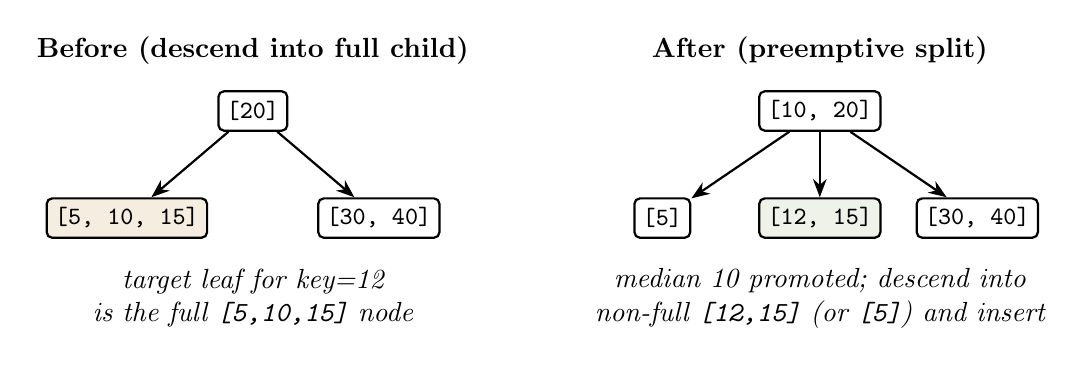
\begin{tikzpicture}[
    btnode/.style={draw, thick, rectangle, rounded corners=2pt,
                   inner sep=3pt, font=\small\ttfamily,
                   minimum height=5mm},
    btedge/.style={->, >=Stealth, thick},
    yscale=0.85,
]
% --- BEFORE frame ---
\node[font=\bfseries] at (-3.6, 3.5) {Before (descend into full child)};
\node[btnode] (b-r) at (-3.6, 2.6) {[20]};
\node[btnode, fill=warnBack] (b-c) at (-5.2, 1.0) {[5, 10, 15]};
\node[btnode] (b-c2) at (-2.0, 1.0) {[30, 40]};
\draw[btedge] (b-r) -- (b-c);
\draw[btedge] (b-r) -- (b-c2);
\node[font=\itshape, align=center] at (-3.6, -0.2)
    {target leaf for key=12\\is the full \texttt{[5,10,15]} node};

% --- AFTER frame ---
\node[font=\bfseries] at (3.6, 3.5) {After (preemptive split)};
\node[btnode] (a-r) at (3.6, 2.6) {[10, 20]};
\node[btnode] (a-l) at (1.6, 1.0) {[5]};
\node[btnode, fill=defnBack] (a-m) at (3.6, 1.0) {[12, 15]};
\node[btnode] (a-rh) at (5.6, 1.0) {[30, 40]};
\draw[btedge] (a-r) -- (a-l);
\draw[btedge] (a-r) -- (a-m);
\draw[btedge] (a-r) -- (a-rh);
\node[font=\itshape, align=center] at (3.6, -0.2)
    {median 10 promoted; descend into\\non-full \texttt{[12,15]} (or
     \texttt{[5]}) and insert};
\end{tikzpicture}
\end{center}

The full \texttt{[5,10,15]} child is split \emph{before} we descend
into it: median 10 moves up to the parent (which had room because
\textbf{we already split it on the way down if it had been full}),
and we now have two non-full children to choose from. The new key
12 goes into \texttt{[12, 15]} via \texttt{btreeInsertNonFull}.

\begin{examplebox}
\textbf{Insert sequence into an empty B-tree of order 4.} We insert
the keys $10, 20, 30, 40, 5, 15, 25, 35, 45$ in order, watching the
preemptive-split invariant in action.

\textbf{Frame 1 (after 10, 20, 30):} root is a single 3-key node.
\begin{center}\texttt{[10, 20, 30]}\end{center}

\textbf{Frame 2 (insert 40 --- root is full).} CLRS variant:
\texttt{btreeInsertCLRS} sees \texttt{t.root->isFull()}, allocates a
new root, makes the old root its only child, then calls
\texttt{btreeSplitChild(newRoot, 0)}. The median 20 moves up.
Then \texttt{btreeInsertNonFull(newRoot, 40)} descends right and
inserts:
\begin{center}\begin{tabular}{c}
    \texttt{[20]} \\
    $/ \quad \backslash$ \\
    \texttt{[10]} \quad \texttt{[30, 40]}
\end{tabular}\end{center}

\textbf{Frame 3 (insert 5):} root \texttt{[20]} not full; descend
left into \texttt{[10]} (not full); insert in sorted order.
\begin{center}\begin{tabular}{c}
    \texttt{[20]} \\
    $/ \quad \backslash$ \\
    \texttt{[5, 10]} \quad \texttt{[30, 40]}
\end{tabular}\end{center}

\textbf{Frame 4 (insert 15):} root not full; descend left;
\texttt{[5, 10]} not full; insert. Then descend right path with the
\textbf{next} insertion (25): \texttt{[5, 10, 15]} would be full
on the way; we don't touch it because 25 goes right.
\begin{center}\begin{tabular}{c}
    \texttt{[20]} \\
    $/ \quad \backslash$ \\
    \texttt{[5, 10, 15]} \quad \texttt{[25, 30, 40]}
\end{tabular}\end{center}
(Inserting 25 into \texttt{[30, 40]} just shifts in place; that
node is still non-full at 3 keys.)

\textbf{Frame 5 (insert 35 --- right child is full).} Descent reaches
the root \texttt{[20]} (not full) and prepares to descend right. The
right child \texttt{[25, 30, 40]} is full, so
\texttt{btreeSplitChild(root, 1)} runs first: median 30 moves up to
the root, splitting the child into \texttt{[25]} and \texttt{[40]}.
\textbf{Then} we descend into the appropriate half (35 is between 30
and 40, so we land in \texttt{[40]}) and insert:
\begin{center}\begin{tabular}{c}
    \texttt{[20, 30]} \\
    $/ \quad | \quad \backslash$ \\
    \texttt{[5, 10, 15]} \quad \texttt{[25]} \quad \texttt{[35, 40]}
\end{tabular}\end{center}

\textbf{Frame 6 (insert 45):} root \texttt{[20, 30]} not full;
descend right into \texttt{[35, 40]}; not full; insert.
\begin{center}\begin{tabular}{c}
    \texttt{[20, 30]} \\
    $/ \quad | \quad \backslash$ \\
    \texttt{[5, 10, 15]} \quad \texttt{[25]} \quad \texttt{[35, 40, 45]}
\end{tabular}\end{center}

Two splits in 9 inserts; both happened \emph{before} the descent
that needed them. No split ever propagated upward retroactively.
\end{examplebox}

\section{11.4 Rotations and Fusion}

Removal is the hard half of any balanced tree. For B-trees, the two tools are \textbf{rotation} (borrow a key from a sibling) and \textbf{fusion} (merge three nodes into one -- the inverse of split).

\subsection*{The CLRS 4-case deletion taxonomy}

CLRS Ch.~18.3 organises B-tree deletion into four cases, branching
on \emph{where} the key sits and \emph{whether} the path to it is
``safe to descend'' (every non-root node has $\ge t$ keys, i.e., one
above the floor, so we can remove a key without underflowing). The
taxonomy is the canonical mental model for the deletion algorithm:

\begin{defnbox}
\textbf{B-TREE-DELETE cases (CLRS 18.3).} Let $t = \lceil K/2 \rceil$
(the minimum-degree parameter). To delete \texttt{key} from the
B-tree rooted at \texttt{r}:

\begin{itemize}[leftmargin=*]
    \item \textbf{Case 1.} \texttt{key} is in node $x$ \emph{and} $x$
          is a leaf. Just delete \texttt{key} from $x$ (shift
          neighbours left). Safe by the descent invariant: $x$ had
          $\ge t$ keys before this operation.
    \item \textbf{Case 2.} \texttt{key} is in internal node $x$ at
          slot $i$. Three subcases on the children $y =
          x\rightarrow$\texttt{children[i]} (predecessor side) and
          $z = x\rightarrow$\texttt{children[i+1]} (successor side):
          \begin{itemize}
              \item \textbf{2a.} $y$ has $\ge t$ keys. Find the
                    \emph{predecessor} (max key in subtree of $y$),
                    swap into $x$'s slot $i$, and recursively delete
                    the predecessor from $y$.
              \item \textbf{2b.} $y$ has $t-1$ keys but $z$ has
                    $\ge t$ keys. Mirror: use the \emph{successor}
                    from $z$.
              \item \textbf{2c.} Both $y$ and $z$ have $t-1$ keys.
                    \textbf{Fuse} them with the separator key
                    \texttt{key} in between, producing one node with
                    $2t-1$ keys, then recursively delete \texttt{key}
                    from the fused node. (\texttt{key} is now in
                    that node; recursion lands in case 1 or recurses
                    further.)
          \end{itemize}
    \item \textbf{Case 3.} \texttt{key} is \emph{not} in node $x$;
          the descent must continue into child
          $c_i = x\rightarrow$\texttt{children[i]}. Before
          descending, ensure $c_i$ has $\ge t$ keys (so the
          recursive call inside $c_i$'s subtree can complete
          safely):
          \begin{itemize}
              \item \textbf{3a.} $c_i$ has $t-1$ keys but an
                    immediate sibling has $\ge t$ keys. \textbf{Rotate}
                    a key from the sibling through $x$ into $c_i$.
              \item \textbf{3b.} $c_i$ has $t-1$ keys and both
                    immediate siblings have $t-1$ keys. \textbf{Fuse}
                    $c_i$ with one sibling and the separator key from
                    $x$.
          \end{itemize}
          Then descend into the (now-safe) child and recurse.
    \item \textbf{Special case:} the root drops to 0 keys after a
          fusion. In that case, the tree shrinks: the new root
          becomes the (unique) child. \textbf{This is the only way a
          B-tree's height shrinks.}
\end{itemize}
\end{defnbox}

\begin{notebox}
\textbf{Why preemptive merge during descent?} Same engineering move
as preemptive split for insertion. A naive ``delete the leaf key,
then fix any underflow on the way back up'' algorithm requires either
parent pointers or a return-from-recursion second pass. By
preemptively rotating-or-fusing on the way down (case 3a / 3b
\emph{before} entering the child), we maintain the invariant ``every
node we touch has $\ge t$ keys'' --- the deletion at the leaf can
proceed without underflowing, no upward recursion needed. As with
preemptive split, we do a small amount of work (some rotations or
fuses) that might not have been strictly necessary, in exchange for
a single-pass algorithm with no parent pointers.
\end{notebox}

\subsection*{Rotation}

\begin{defnbox}
\textbf{Rotation (B-tree sense).} Move one key from a source node, \emph{through the parent}, into a sibling. The source loses a key, the sibling gains a key, and the parent key that was between them is swapped out for a key from the source.
\end{defnbox}

\begin{ideabox}
This is \emph{not} the same as the AVL/red-black rotation. AVL rotations re-parent subtrees to restore a height balance. B-tree rotations \textbf{redistribute keys across sibling nodes} -- the tree shape doesn't change, only which key lives in which node.
\end{ideabox}

\subsection*{Right rotation on \texttt{node}}

Takes a key from \texttt{node}'s left sibling, moves the parent separator key into \texttt{node}, and pushes the left sibling's rightmost key up to fill the separator slot. Result: the left sibling loses one key, \texttt{node} gains one.

\subsection*{Left rotation on \texttt{node}}

Mirror image: takes a key from \texttt{node}'s right sibling.

\begin{lstlisting}[basicstyle=\ttfamily\small,frame=single]
// Illustrative form. A "rotation on node X" in this context means
// "give X one more key by borrowing from a sibling through the parent."
void btreeRotateLeft(BTreeNode* node) {
    BTreeNode* leftSib = getLeftSibling(node);
    int parentKey = getParentKeyLeftOfChild(node->parent, node);
    addKeyAndChild(leftSib, parentKey, node->children[0]);
    setParentKeyLeftOfChild(node->parent, node, node->keys[0]);
    removeKey(node, 0);
}
\end{lstlisting}

\subsection*{Fusion}

\begin{defnbox}
\textbf{Fusion.} Merge a parent separator key with two single-key adjacent siblings into one fused 3-key node. \emph{The inverse of split.}
\end{defnbox}

\begin{center}
\begin{tabular}{lll}
Before fusion & $\to$ & After fusion \\
\texttt{[L]} $\cdot$ (parent sep $M$) $\cdot$ \texttt{[R]} & $\to$ & \texttt{[L, M, R]} \\
\end{tabular}
\end{center}

The parent loses a key (and a child pointer); the fused node has three keys. Fusion is used when neither sibling has a spare key to rotate.

\subsection*{Root fusion -- a special case}

When the root has 1 key and both its children have 1 key each, no rotation is possible and ordinary fusion would empty the parent. Instead, the three keys are combined into a \emph{new root} of three keys, and the tree shrinks in height by 1:

\begin{ideabox}
Root fusion is the only way a B-tree shrinks in height, mirroring how root split is the only way it grows. Every other operation happens at leaf level or via local restructuring.
\end{ideabox}

\subsection*{Picture: rotation from sibling vs.\ fusion with sibling}

Cases 3a and 3b of the deletion taxonomy decide between the two
deletion-prep strategies. The diagrams below show both moves on the
same starting configuration --- the deficient child \texttt{[c]} has
$t-1 = 1$ key (order $K=4$), and we need to ensure it has at least
$t = 2$ before descending into it.

\begin{center}
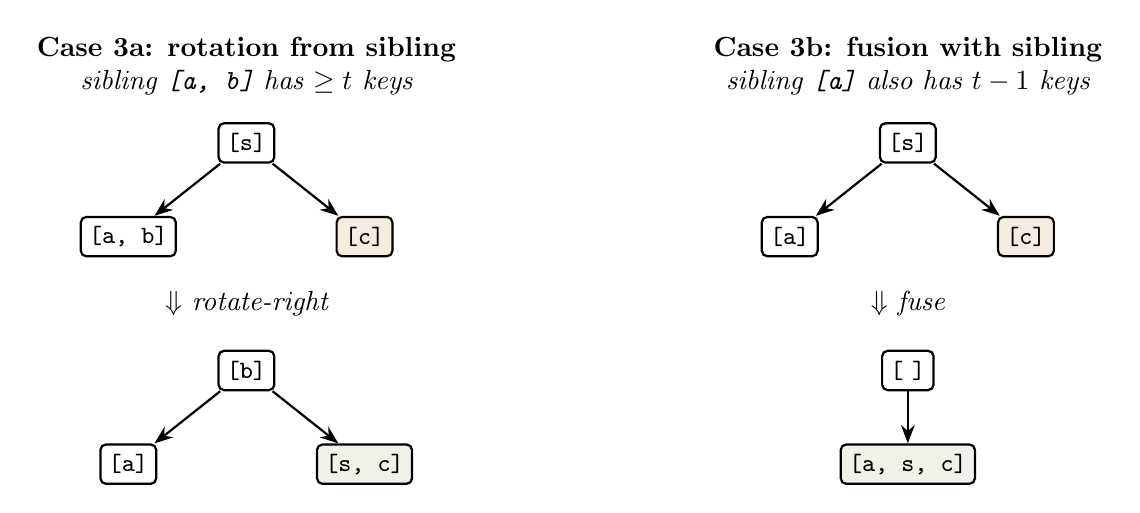
\begin{tikzpicture}[
    btnode/.style={draw, thick, rectangle, rounded corners=2pt,
                   inner sep=3pt, font=\small\ttfamily,
                   minimum height=5mm},
    btedge/.style={->, >=Stealth, thick},
    yscale=0.85,
]
% --- Case 3a: rotation from left sibling (sibling has spare key) ---
\node[font=\bfseries] at (-4.2, 4.4) {Case 3a: rotation from sibling};
\node[font=\itshape, align=center] at (-4.2, 3.9)
    {sibling \texttt{[a, b]} has $\ge t$ keys};

\node[btnode] (a-p) at (-4.2, 3.0) {[s]};
\node[btnode] (a-l) at (-5.7, 1.6) {[a, b]};
\node[btnode, fill=warnBack] (a-c) at (-2.7, 1.6) {[c]};
\draw[btedge] (a-p) -- (a-l);
\draw[btedge] (a-p) -- (a-c);

\node[font=\itshape] at (-4.2, 0.6) {$\Downarrow$ rotate-right};

\node[btnode] (a-p2) at (-4.2, -0.4) {[b]};
\node[btnode] (a-l2) at (-5.7, -1.8) {[a]};
\node[btnode, fill=defnBack] (a-c2) at (-2.7, -1.8) {[s, c]};
\draw[btedge] (a-p2) -- (a-l2);
\draw[btedge] (a-p2) -- (a-c2);

% --- Case 3b: fusion with sibling (both siblings minimal) ---
\node[font=\bfseries] at (4.2, 4.4) {Case 3b: fusion with sibling};
\node[font=\itshape, align=center] at (4.2, 3.9)
    {sibling \texttt{[a]} also has $t-1$ keys};

\node[btnode] (b-p) at (4.2, 3.0) {[s]};
\node[btnode] (b-l) at (2.7, 1.6) {[a]};
\node[btnode, fill=warnBack] (b-c) at (5.7, 1.6) {[c]};
\draw[btedge] (b-p) -- (b-l);
\draw[btedge] (b-p) -- (b-c);

\node[font=\itshape] at (4.2, 0.6) {$\Downarrow$ fuse};

\node[btnode] (b-p2) at (4.2, -0.4) {[\,\,]};
\node[btnode, fill=defnBack] (b-fused) at (4.2, -1.8) {[a, s, c]};
\draw[btedge] (b-p2) -- (b-fused);
\end{tikzpicture}
\end{center}

\textbf{Reading the two cases.} The shaded child is the one we're
about to descend into; we must raise its key count above the floor
first.

\begin{itemize}[leftmargin=*]
    \item \textbf{Case 3a (left).} Sibling \texttt{[a, b]} has
          $\ge t$ keys. \textbf{Rotate-right}: $b$ stays in the left
          sibling, $a$? No --- the parent separator $s$ comes down
          into $c$, and the sibling's rightmost key $b$ moves up to
          take $s$'s place. (Mirror of left-rotation when the spare
          key is in the right sibling.) The child gains one key,
          the sibling loses one, the parent's key changes but its
          count stays the same.
    \item \textbf{Case 3b (right).} Both siblings have only $t - 1$
          keys; no rotation possible. \textbf{Fuse} the parent's
          separator $s$ with both children into one node of
          $2t - 1$ keys. The parent loses one key + one child
          pointer. If the parent was the root and is now empty,
          the fused node becomes the new root --- the only way a
          B-tree shrinks in height (mirror of root-split being the
          only way it grows).
\end{itemize}

\subsection*{Visualizing split vs.\ fusion}

\begin{center}
\begin{tabular}{lcc}
\hline
Operation & Effect on height & Inverse of \\
\hline
Root split & +1 & Root fusion \\
Internal split & 0 & Internal fusion \\
Right rotation & 0 & Left rotation (roughly) \\
\hline
\end{tabular}
\end{center}

The symmetry is beautiful: \emph{every modification to a B-tree is either a rotation (constant-cost redistribution) or a split/fuse (constant-cost restructuring)}. Both are strictly local.

\section{11.5 Removal}

\subsection*{The same dual-pass idea as insertion}

Insertion used \emph{preemptive split}: any full node seen on the way down gets split before we touch it, guaranteeing the target leaf has room.

Removal uses the mirror: \textbf{preemptive merge}. Any single-key non-root node seen on the way down gets merged (via rotation or fusion) to have $\geq 2$ keys before we touch it. That guarantees the target leaf has $\geq 2$ keys and can give one up.

\begin{ideabox}
The parallel is exact. Inserting needs non-full leaves; removing needs non-minimal leaves. Both algorithms do a single downward pass, maintaining the invariant that the current node is safe to modify.
\end{ideabox}

\subsection*{The merge procedure}

Given a 1-key non-root node whose parent has $\geq 2$ keys, merge as follows:

\begin{lstlisting}[basicstyle=\ttfamily\small,frame=single]
BTreeNode* btreeMerge(BTreeNode* node) {
    BTreeNode* leftSib  = getLeftSibling(node);
    BTreeNode* rightSib = getRightSibling(node);

    // Preference 1: rotate from a sibling with a spare key.
    if (leftSib && leftSib->numKeys >= 2) {
        btreeRotateRight(leftSib);   // one of leftSib's keys flows into node
    } else if (rightSib && rightSib->numKeys >= 2) {
        btreeRotateLeft(rightSib);
    } else {
        // Preference 2: fuse with a 1-key adjacent sibling.
        if (!leftSib) node = btreeFuse(node, rightSib);
        else          node = btreeFuse(leftSib, node);
    }
    return node;
}
\end{lstlisting}

\subsection*{Leaf case vs.\ internal case}

\textbf{Leaf removal.} Once preemptive merging has guaranteed the leaf has $\geq 2$ keys, just splice the key out and shift neighbors left.

\textbf{Internal removal.} Replace the key with its \emph{successor} (the minimum key in its right subtree) -- just like BST removal. But now we have to recursively remove the successor, which \emph{is} in a leaf. The remove call:

\begin{enumerate}[leftmargin=*]
    \item Find and remember the successor key.
    \item Recursively remove the successor (which triggers a leaf removal, safe after merging).
    \item Swap the saved successor key into the original internal node's position.
\end{enumerate}

\begin{lstlisting}[basicstyle=\ttfamily\small,frame=single]
bool btreeRemove(BTree& t, int key) {
    // Special case: single-key leaf root.
    if (t.root->isLeaf() && t.root->numKeys == 1 && t.root->keys[0] == key) {
        delete t.root; t.root = nullptr; return true;
    }

    BTreeNode* cur = t.root;
    while (cur) {
        // Preemptive merge: no 1-key non-root nodes on our path.
        if (cur->numKeys == 1 && cur != t.root)
            cur = btreeMerge(cur);

        int idx = indexOfKey(cur, key);
        if (idx != -1) {
            if (cur->isLeaf()) {
                removeKey(cur, idx);
                return true;
            }
            // Internal: swap with min of right child, then remove the min.
            BTreeNode* rightChild = cur->children[idx + 1];
            int replacement = btreeGetMinKey(rightChild);
            btreeRemove(t, replacement);
            btreeKeySwap(t.root, key, replacement);
            return true;
        }
        cur = btreeNextNode(cur, key);   // descend toward the target
    }
    return false;   // not found
}
\end{lstlisting}

\subsection*{Cost}

Same as insertion: $O(K \log_K n) = O(\log n)$. Single downward pass, constant work per level.

\subsection*{Why preemptive merging is elegant}

\begin{ideabox}
A naive removal needs recursion back up the tree when a leaf underflows. Preemptive merging eliminates upward recursion entirely by strengthening every node \emph{before} it gets weakened. It's the same engineering move as preemptive split on insert -- trade a tiny bit of extra work (merging nodes that might not have needed it) for a much simpler one-pass algorithm.
\end{ideabox}

\subsection*{B+ trees -- the production refinement}

Real databases and filesystems use \textbf{B+ trees}, not plain
B-trees. The variant changes \emph{where data lives} and adds a
linked-list-of-leaves structure on top. The algorithms (search,
insert, preemptive split, preemptive merge, rotate, fuse) adapt
directly --- the only change is that internal nodes hold routing
keys but no values, and leaves chain to their right neighbours.

\begin{defnbox}
\textbf{B+ tree.} A B-tree where:
\begin{itemize}[leftmargin=*]
    \item \textbf{Data only at leaves.} Every record (key, value)
          pair lives in a leaf. Internal nodes hold \emph{routing
          keys} only --- copies of leaf keys used to decide which
          subtree to descend into. A routing key in an internal node
          is duplicated in some leaf below it (this is the trade for
          higher fanout).
    \item \textbf{Linked leaves.} Each leaf has a
          \texttt{next} pointer to its right sibling at the leaf
          level (some implementations also chain backward). Range
          scans walk the linked list rather than re-descending from
          the root.
    \item \textbf{Higher fanout.} Internal nodes carry only keys +
          child pointers --- no values --- so more keys fit per
          page. For 4\,KB pages with 8-byte keys + 8-byte child
          pointers, a B+ tree internal node holds $\sim 256$ keys
          while a same-page B-tree (with embedded values, say 64
          bytes each) holds $\sim 50$ keys.
\end{itemize}
\end{defnbox}

\subsection*{B-tree vs B+ tree --- side by side}

\begin{center}
\begin{tabular}{lll}
\hline
Feature & Classic B-tree & B+ tree \\
\hline
Where values live & internal + leaves & leaves only \\
Routing keys & not duplicated & duplicated at leaf \\
Internal-node fanout & moderate & high (no values) \\
Range scan & in-order traversal $O(R \log_K n)$ & leaf walk $O(R)$ \\
Sequential scan & re-descend per row & one leaf walk \\
Point-query depth & may stop at internal & always reaches leaf \\
Production use & rare today & standard everywhere \\
Insert / delete algorithm & as in \S11.3 / \S11.5 & \emph{identical} (with leaf-link bookkeeping) \\
\hline
\end{tabular}
\end{center}

The picture: same conceptual tree shape, but data + links live at
the leaf level only.

\begin{center}
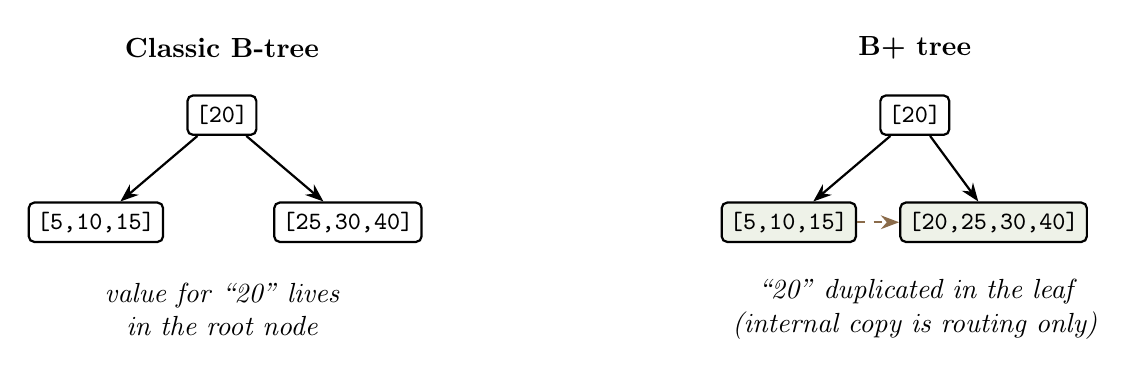
\begin{tikzpicture}[
    btnode/.style={draw, thick, rectangle, rounded corners=2pt,
                   inner sep=3pt, font=\small\ttfamily,
                   minimum height=5mm},
    btleaf/.style={btnode, fill=defnBack},
    btedge/.style={->, >=Stealth, thick},
    bplink/.style={->, >=Stealth, thick, dashed, accent},
    yscale=0.85,
]
% --- LEFT: classic B-tree ---
\node[font=\bfseries] at (-4.4, 3.6) {Classic B-tree};
\node[btnode] (l-r) at (-4.4, 2.6) {[20]};
\node[btnode] (l-l) at (-6.0, 1.0) {[5,10,15]};
\node[btnode] (l-rh) at (-2.8, 1.0) {[25,30,40]};
\draw[btedge] (l-r) -- (l-l);
\draw[btedge] (l-r) -- (l-rh);
\node[font=\itshape, align=center] at (-4.4, -0.3)
    {value for ``20'' lives\\in the root node};

% --- RIGHT: B+ tree ---
\node[font=\bfseries] at (4.4, 3.6) {B+ tree};
\node[btnode] (r-r) at (4.4, 2.6) {[20]};
\node[btleaf] (r-l) at (2.8, 1.0) {[5,10,15]};
\node[btleaf] (r-m) at (5.4, 1.0) {[20,25,30,40]};
\draw[btedge] (r-r) -- (r-l);
\draw[btedge] (r-r) -- (r-m);
\draw[bplink] (r-l) -- (r-m);
\node[font=\itshape, align=center] at (4.4, -0.3)
    {``20'' duplicated in the leaf\\(internal copy is routing only)};
\end{tikzpicture}
\end{center}

\begin{notebox}
\textbf{Why B+ wins for databases.} A point query on a B+ tree always
descends to a leaf (one extra cache line vs the classic B-tree's
optional early-stop), but the win comes elsewhere: a range query
\texttt{SELECT * WHERE x BETWEEN 100 AND 200} descends once to find
$x = 100$ and then walks the leaf linked list emitting tuples until
$x > 200$. No re-descent per tuple, $O(R)$ in the result-set size
$R$, and the leaf walk is sequential disk access (the OS prefetcher
loves it). On a classic B-tree, the same query is $O(R \log_K n)$
because in-order successor traversal climbs back up the tree
between leaves.
\end{notebox}

\begin{examplebox}
\textbf{Worked deletion exercising the 4-case CLRS taxonomy
(\S11.4).} We start with a populated B-tree of order $K = 4$
(min-degree $t = 2$) and delete a sequence of keys to hit each case.

\textbf{Starting tree:}
\begin{center}\begin{tabular}{c}
    \texttt{[20, 40]} \\
    $/ \quad | \quad \backslash$ \\
    \texttt{[5, 10, 15]} \quad \texttt{[25, 30, 35]} \quad \texttt{[45, 50, 55]}
\end{tabular}\end{center}

\textbf{Delete 50 (Case 1 --- key in leaf, leaf has $\ge t$ keys).}
The leaf \texttt{[45, 50, 55]} has 3 keys $\ge t = 2$. Direct delete
+ shift:
\begin{center}\begin{tabular}{c}
    \texttt{[20, 40]} \\
    $/ \quad | \quad \backslash$ \\
    \texttt{[5, 10, 15]} \quad \texttt{[25, 30, 35]} \quad \texttt{[45, 55]}
\end{tabular}\end{center}

\textbf{Delete 20 (Case 2a --- internal node, predecessor side has
spare).} Key 20 is at slot 0 of the root. Left child
\texttt{[5, 10, 15]} has 3 keys ($\ge t$). Find predecessor
(\texttt{btreeGetMaxKey} of left subtree = 15), swap into root, then
recursively delete 15 from the leaf (Case 1):
\begin{center}\begin{tabular}{c}
    \texttt{[15, 40]} \\
    $/ \quad | \quad \backslash$ \\
    \texttt{[5, 10]} \quad \texttt{[25, 30, 35]} \quad \texttt{[45, 55]}
\end{tabular}\end{center}

\textbf{Delete 5 (Case 3a --- key not in current node, descent child
needs a key from sibling).} Root \texttt{[15, 40]} doesn't contain 5;
descend left into \texttt{[5, 10]}. That child has $t - 1 = 1$ keys?
No --- it has 2 keys, so the descent is safe. (We're at the floor's
threshold. Some implementations preemptively rotate here; CLRS waits
until the child is at exactly $t - 1 = 1$ key before fixing.)
Continue: in the leaf, delete 5 (Case 1):
\begin{center}\begin{tabular}{c}
    \texttt{[15, 40]} \\
    $/ \quad | \quad \backslash$ \\
    \texttt{[10]} \quad \texttt{[25, 30, 35]} \quad \texttt{[45, 55]}
\end{tabular}\end{center}

\textbf{Delete 10 (Case 3a --- now the leaf is at the floor).}
Descent reaches root \texttt{[15, 40]}; left child is \texttt{[10]}
with $t - 1 = 1$ key --- below the safe threshold for descent.
Sibling \texttt{[25, 30, 35]} has $\ge t$ keys, so \textbf{rotate}
the separator 15 down into the left child and pull the smallest
sibling key 25 up to the root:
\begin{center}\begin{tabular}{c}
    \texttt{[25, 40]} \\
    $/ \quad | \quad \backslash$ \\
    \texttt{[10, 15]} \quad \texttt{[30, 35]} \quad \texttt{[45, 55]}
\end{tabular}\end{center}
Now descend (safe) into the left child and delete 10 (Case 1):
\begin{center}\begin{tabular}{c}
    \texttt{[25, 40]} \\
    $/ \quad | \quad \backslash$ \\
    \texttt{[15]} \quad \texttt{[30, 35]} \quad \texttt{[45, 55]}
\end{tabular}\end{center}

\textbf{Delete 25 (Case 2c --- internal node, both adjacent children
minimal).} Key 25 is at slot 0 of the root. Left child \texttt{[15]}
has $t - 1 = 1$ key, right child \texttt{[30, 35]} has 2 keys --- not
both minimal, so this falls into \textbf{Case 2b} (predecessor
minimal but successor has spare). Use the successor: minimum of
\texttt{[30, 35]} = 30, swap into root, recursively delete 30 from
right-sibling leaf (Case 1):
\begin{center}\begin{tabular}{c}
    \texttt{[30, 40]} \\
    $/ \quad | \quad \backslash$ \\
    \texttt{[15]} \quad \texttt{[35]} \quad \texttt{[45, 55]}
\end{tabular}\end{center}

\textbf{Delete 35 (Case 3b --- descent child minimal, both siblings
minimal).} Root \texttt{[30, 40]} doesn't contain 35; descend into
middle child \texttt{[35]}. That child has 1 key, both immediate
siblings (\texttt{[15]} and \texttt{[45, 55]}) --- the right sibling
has $\ge t$ keys, so this is actually \textbf{Case 3a}: rotate from
right sibling. Pull separator 40 down, pull smallest sibling key 45
up:
\begin{center}\begin{tabular}{c}
    \texttt{[30, 45]} \\
    $/ \quad | \quad \backslash$ \\
    \texttt{[15]} \quad \texttt{[35, 40]} \quad \texttt{[55]}
\end{tabular}\end{center}
Now descend safely; delete 35 from middle leaf:
\begin{center}\begin{tabular}{c}
    \texttt{[30, 45]} \\
    $/ \quad | \quad \backslash$ \\
    \texttt{[15]} \quad \texttt{[40]} \quad \texttt{[55]}
\end{tabular}\end{center}

\textbf{Delete 40 (true Case 3b --- all three children at the
floor).} Root \texttt{[30, 45]}; key 40 sits between the two
separators, so descent goes into middle child \texttt{[40]}.
Middle has $t - 1 = 1$, left and right both have $t - 1 = 1$ ---
both siblings minimal. \textbf{Fuse}: pick the left sibling +
separator 30, fuse with middle into one node \texttt{[15, 30, 40]}.
The root loses key 30 and child pointer:
\begin{center}\begin{tabular}{c}
    \texttt{[45]} \\
    $/ \quad \backslash$ \\
    \texttt{[15, 30, 40]} \quad \texttt{[55]}
\end{tabular}\end{center}
Now descend into \texttt{[15, 30, 40]} (3 keys, safe) and delete 40:
\begin{center}\begin{tabular}{c}
    \texttt{[45]} \\
    $/ \quad \backslash$ \\
    \texttt{[15, 30]} \quad \texttt{[55]}
\end{tabular}\end{center}

Across 7 deletions we exercised all four cases (1, 2a/2b, 3a, 3b)
and never recursed back up the tree. Single downward pass per
delete, in line with the preemptive-merge invariant.
\end{examplebox}

\section{11.6 Memory hierarchy and B-tree variants}

The basic B-tree of \S11.1--\S11.5 is the foundation; production
systems layer on variants that target different points in the
memory hierarchy.

\subsection*{2-3-4 trees and red-black trees are the same data structure}

\begin{notebox}
\textbf{The 2-3-4 $\leftrightarrow$ red-black equivalence
(CLRS Ch.~13 problem 13-4).} Every red-black tree corresponds
\emph{exactly} to a 2-3-4 tree under the following rule:
\begin{itemize}[leftmargin=*]
    \item A 2-node in the 2-3-4 tree becomes a black node in the RB
          tree (with 2 black/red children handled by the recursion).
    \item A 3-node becomes a black node with one red child (the red
          child contributes the second key).
    \item A 4-node becomes a black node with two red children
          (the red children contribute the second and third keys).
\end{itemize}
The black-height of the RB tree equals the height of the 2-3-4 tree;
red-black insertion / deletion fixups exactly emulate 2-3-4 split /
fusion. AVL is the only major balanced-binary-tree that doesn't have
a clean 2-3-4 mapping --- it sits in a different equivalence class.
This explains why \textbf{ch.~9} red-black insert/delete had so many
cases (red uncle / black uncle / left/right zig-zag): it's
\textbf{the 2-3-4 algorithm in disguise}, with the cases being the
``which colour pattern correspond to which 2-3-4 node?'' decoding.
\end{notebox}

\subsection*{Cache-oblivious B-trees}

\begin{notebox}
\textbf{Cache-oblivious B-trees (Bender, Demaine, Farach-Colton
2000).} The classic B-tree achieves $O(\log_B n)$ block transfers
\emph{when you know $B$} (the block size --- you tune the order $K$
to match). What if your code has to run well across L1, L2, L3,
DRAM, NVMe, and disk simultaneously, where each level has a
different $B$? You'd need a different B-tree per level.

The \textbf{van Emde Boas layout} gives a single tree structure that
achieves $O(\log_B n)$ transfers \emph{for every $B$ simultaneously},
without the algorithm knowing $B$. Recursively split a height-$h$
tree into a top half (height $h/2$) and bottom half (height $h/2$),
laying them out contiguously in memory; recurse to the leaves. The
analysis is non-trivial but the layout is what every modern
``cache-oblivious'' data structure uses.

Practical impact: production engines (e.g., Google's LevelDB
internals, recent academic OLTP work) sometimes prefer
cache-oblivious layouts to portable B-trees because they don't have
to be retuned per platform.
\end{notebox}

\subsection*{LSM-trees: the write-optimized alternative}

\begin{notebox}
\textbf{Log-Structured Merge trees (O'Neil, Cheng, Gawlick, O'Neil
1996).} B-trees are read-optimized: a random read costs
$O(\log_B n)$ block transfers, but a random insert costs the same
because the tree must be modified in place at the leaf. For
write-heavy workloads (logging, time-series, key-value stores
serving high writes), the in-place update is the bottleneck.

\textbf{LSM-trees} buffer writes in memory in a sorted in-memory
structure (often a skip list or red-black tree, called the
\emph{memtable}); when the memtable hits a size threshold, it is
flushed to disk as a sorted immutable file (an \emph{SSTable}).
Reads check the memtable first, then check on-disk SSTables in
reverse-chronological order. Background compaction merges SSTables
to keep read amplification bounded.

LSM-trees have higher write throughput (sequential writes are
roughly $100\times$ faster than random writes on disk and SSDs)
and worse read latency (multiple SSTables may need to be checked
per key). Production: \textbf{LevelDB}, \textbf{RocksDB},
\textbf{Cassandra}, \textbf{HBase}, \textbf{ScyllaDB}. The
B-tree-vs-LSM choice is the canonical read-vs-write trade-off in
storage system design.
\end{notebox}

\subsection*{Other variants worth pointing at}

\begin{notebox}
\textbf{Fractal trees / $B^\varepsilon$-trees} (Brodal \& Fagerberg
2003, Bender et al. 2007): an asymptotic improvement on B-trees that
trades some read latency for far better insert throughput, by
buffering inserts at internal nodes. The basis of the
\textbf{TokuDB} / \textbf{TokuMX} storage engine (now part of
Percona).

\textbf{Bw-trees} (Levandoski, Lomet, Sengupta 2013): a lock-free
B+-tree variant designed for many-core in-memory databases. The
basis of \textbf{Microsoft Hekaton}'s in-memory engine and influential
in modern OLTP storage.

\textbf{Copy-on-write B-trees}: every modification creates a new
path from leaf to root, leaving the old tree untouched.
\textbf{Btrfs} and \textbf{ZFS} are built on this, and it
underpins the snapshot / clone primitives those filesystems
expose.
\end{notebox}

\section{11.7 Production references and further reading}

\begin{notebox}
\textbf{Where B-trees show up in real systems.}
\begin{itemize}[leftmargin=*]
    \item \textbf{SQLite.} B+ tree, default page size 4096 bytes
          (configurable 512--65536). Both table indexes and the
          rowid B+ tree storing the table itself.
    \item \textbf{PostgreSQL.} \texttt{btree} access method (the
          default for any \texttt{CREATE INDEX} that doesn't say
          otherwise); also has \texttt{gist} (R-tree-flavored, for
          spatial data) and \texttt{gin} (inverted index, for
          full-text and array containment). The \texttt{btree}
          implementation is a B+ tree with concurrent-access
          mechanics (Lehman--Yao 1981 right-link technique).
    \item \textbf{MySQL InnoDB.} Clustered B+ tree on the primary
          key (table data lives at the leaves); secondary indexes
          are separate B+ trees that point at primary-key values.
          Default page size 16\,KB.
    \item \textbf{Linux ext4.} \texttt{htree} variant for directory
          entries (an HTree is a B-tree-like hashed-index structure
          --- enough fanout to keep large directories fast).
    \item \textbf{Btrfs.} Copy-on-write B+ trees throughout the
          filesystem (extent allocation, file-system tree,
          subvolumes, checksums). The ``B'' is for B-tree.
    \item \textbf{git packfile (.idx).} \emph{Not} a B-tree --- a
          sorted-array index with a small fanout table at the front
          for log-time lookup. Worth contrasting: git's access
          pattern is read-mostly, append-only, and doesn't need
          range queries; the simpler structure is the right call.
    \item \textbf{LSM-tree-on-top engines.} \textbf{LevelDB},
          \textbf{RocksDB}, \textbf{Cassandra}, \textbf{HBase},
          \textbf{ScyllaDB}. Don't use B-trees on disk
          (write-optimised), but the in-memory memtable is often a
          skip list or red-black tree, and on-disk SSTables are
          sorted-string-table files that get B-tree-like indexes
          themselves.
\end{itemize}

\textbf{Canonical references.}
\begin{itemize}[leftmargin=*]
    \item \textbf{CLRS Ch.~18} (B-Trees). The textbook treatment;
          minimum-degree $t$ convention, B-TREE-SEARCH /
          SPLIT-CHILD / INSERT-NONFULL, the 4-case deletion
          taxonomy. The version cited throughout this chapter.
    \item \textbf{Goetz Graefe, ``Modern B-Tree Techniques''}
          (Foundations and Trends in Databases, 2010). 200-page
          monograph covering production-engineering details:
          concurrent access, write-ahead logging integration,
          bulk-loading, prefix B-trees, and partitioning. The
          industry reference.
    \item \textbf{Knuth, TAOCP vol. 3 \S6.2.4.} The original
          treatment of multiway trees, including Knuth's bottom-up
          insert (the ``lazy alternative'' warnbox in \S11.3).
    \item \textbf{Bender, Demaine, Farach-Colton, ``Cache-Oblivious
          B-Trees''} (FOCS 2000). The van Emde Boas layout result
          referenced in \S11.6.
    \item \textbf{Bayer \& McCreight, ``Organization and Maintenance
          of Large Ordered Indexes''} (1972). The original B-tree
          paper.
\end{itemize}
\end{notebox}

\begin{ideabox}
\textbf{Chapter takeaway.} A B-tree is a balanced search tree where
\emph{balance via fanout, not branching} is the operating principle:
each non-root node carries between $\lceil K/2 \rceil - 1$ and
$K - 1$ keys, which gives $h = O(\log_K n)$ and ties tree height
directly to the memory hierarchy --- one block per level by design.
The chapter unifies under four sub-algorithms, all single-pass:
\begin{itemize}[leftmargin=*]
    \item \textbf{Search} (\S11.2): in-node scan + single descent
          per level. CPU $O(\log n)$ with binary in-node search;
          disk $O(\log_K n)$ regardless. Same primitive as classic
          BST search, applied per node.
    \item \textbf{Preemptive-split insert} (\S11.3): split full
          nodes \emph{on the way down}; the descent invariant
          ``current node has room'' is preserved.
          \texttt{btreeSplitChild} + \texttt{btreeInsertNonFull}
          together --- one downward pass, no parent pointers, no
          second pass.
    \item \textbf{Preemptive-merge remove} (\S11.4--\S11.5): mirror
          --- rotate-or-fuse on the way down (cases 3a / 3b of the
          CLRS taxonomy) so the leaf to delete from always has
          $\ge t$ keys. Internal-node deletion (case 2) replaces
          the key with a predecessor or successor and recurses
          into a leaf; case 2c fuses the two children when both
          are minimal.
    \item \textbf{Rotation + fusion} (\S11.4): the two
          constant-cost local restructuring primitives both insert
          and remove rely on. Rotation is the inverse of itself
          (left $\leftrightarrow$ right); fusion is the inverse of
          split. Every B-tree modification is one of these four.
\end{itemize}

With $K$ in the hundreds, $\log_K n \le 5$ for billions of keys ---
B-tree lookups are essentially $O(1)$ on any realistic workload, and
that's why every serious storage system in production uses one.

\textbf{Looking ahead.} \textbf{Chapter 12} covers the \emph{set ADT}
in full. The ``does this set contain $x$?'' / ``insert $x$'' /
``remove $x$'' / ``iterate in order'' interface is what B-trees and
B+ trees implement on disk; \texttt{std::set} / \texttt{std::map} use
red-black trees (the in-memory dual --- recall \S11.6's 2-3-4
$\leftrightarrow$ red-black equivalence), Java's \texttt{TreeMap}
likewise, and SQLite / PostgreSQL / InnoDB use B+ trees. The chapter
will frame these as implementation choices for the same ADT.
\textbf{Forward direction beyond cs-300}: the variants in \S11.6
(cache-oblivious B-trees, LSM-trees, fractal trees, Bw-trees) are
where modern storage-system research lives, and Graefe's monograph
(\S11.7) is the entry point.
\end{ideabox}

\end{document}
